\documentclass[letterpaper, 11pt]{article}
\usepackage{comment} % enables the use of multi-line comments (\ifx \fi) 
\usepackage{fullpage} % changes the margin
\usepackage{fancyhdr} % for footerhttps://www.overleaf.com/3039851kkndbp#
\usepackage[UKenglish]{isodate}% http://ctan.org/pkg/isodate for date format
\usepackage{float}%force tables/figs into certain placement
\usepackage{changepage}%for dichotomous key
\usepackage{graphicx}%for figures
\usepackage{subcaption}%for figures
\usepackage{hyperref}%for links
\usepackage[font=small,labelfont=bf]{caption}%for captions
\usepackage[letterpaper,margin=1in]{geometry}
\usepackage{natbib}	%for bibliography
\usepackage{placeins}%prevent images from floating into inappropriate sections

\def\labelitemi{--}

\pagestyle{fancy}
\renewcommand{\headrulewidth}{0pt}

\lhead{}
\chead{}
\rhead{}
\lfoot{ENT 432 (Fall 2016) - Penn State}
\cfoot{}
\rfoot{\thepage}
\renewcommand{\footrulewidth}{0.4pt}
\title{Unit 11 - Hymenoptera}
\author{Andrew R. Deans and Istv\'an Mik\'o}

\begin{document}
\cleanlookdateon %removed ordinal date
\maketitle
\thispagestyle{fancy}
\section*{Introduction}
Today we begin looking at a taxon named \textbf{Holometabola}, which all exhibit a form of development called \textbf{holometaboly}. The immature stage (\textbf{larva}) is quite different, usually, from the imago, and the transition to adulthood takes place in a stage we refer to as the \textbf{pupa}. We'll discuss this life cycle in more detail in a later lecture. This lecture focuses on \textbf{Hymenoptera}, a lineage of almost indescribable diversity (155,000 known species and probably at least a million that need names). Is this the largest order? Possibly. These species, commonly known as sawflies, wasps, bees, and ants, exhibit a broad array of morphologies and life histories. Their ecological and economic importance, as predators (\textit{e.g.}, ants), pollinators (bees), pests (\textit{e.g.}, some herbivorous sawflies), and bio-control agents (numerous parasitic wasps) is enormous. 

The predominant parasitoid/predatory lifestyle amongst the derived lineage, Apocrita, is arguably impacted by the appearance of an evolutionary novelty, the wasp waist. The wasp waist separates the locomotory tagma, the mesosoma, from the tagma of reproduction and digestion, the metasoma; it allows for an exceptionally flexible mechanism to maneuver the sting or egg-laying device (ovipositor). Members of this order can be readily separated from other insects based on the following characteristics:

\begin{itemize}
\item haplodiploidy (males are haploid)
\item smaller hind wings connected to larger fore wings by hook-like spurs (hamuli)
\item transverse and longitudinal veins cannot be differentiated (compare with Odonata and Plecoptera, \textit{e.g.}, where transverse veins are usually less sclerotized and more flexible than longitudinal veins)
\item protibial apical spur and the first basitarsus is modified into an antenna cleaning device
\item abdominal tergite I at least partly fused with metanotum
\end{itemize}

\subsection*{Big picture questions}
Given what you read and discussed in lecture, what adaptations contributed to such a large radiation? How does this diversity look phylogenetically?\\

\noindent{}How do \textbf{idiobiont} parasitoids differ from \textbf{koinobiont}s?\\

\noindent{}Familiarize yourself with the following taxon names, which refer to organisms you are likely to encounter in the northeastern USA and/or which are phylogenetically relevant. Can you describe how these arthropods live (natural history) and roughly how diverse they are? Do you know how they're related to one another? If you had to choose a family to study from the taxa below which one would it be and why?

\begin{enumerate} 
\item Apocrita
\item Aculeata
\item Orussidae
\end{enumerate}

\section*{Materials}
\begin{itemize}
\item specimens (provided)
\item fine forceps, probes (provided)
\item sorting tray, watch glasses, gloves, safety glasses, glycerine, ethanol (provided)
\item pencil/paper for sketches
\end{itemize}

\section*{Safety}
We will be working with sharp tools and insects on pins. Wear your personal protective gear at all times. Specimens are to be returned to their vials after lab, and glycerine and ethanol will be collected for proper disposal or reuse.

\section*{Methods}
Working with a partner, organize your space, specimens, tools, and microscope. Use your probe and forceps to manipulate the specimen. In this lab, however, we will not be dissecting specimens (unless otherwise noted). You can start anywhere in the handout.

\section{Hymenoptera}
\subsection{Non-apocritan Hymenoptera (``Symphyta'')}
\noindent{}\textit{Diagnostic characters:} Body in dorsal view with very little or no constriction near its middle between abdominal segments 1 and 2 (\textit{i.e}., ``wasp waist'' absent; Figure \ref{fig:symphyt1}); cenchrus usually present (arrows in Figure \ref{fig:symphyt1}); fore tibia with two apical spurs; never less than 3 mm in length; first abdominal tergite usually divided medially.\\

\noindent{}\textit{Natural history:} Non-apocritans, known commonly as ``sawflies'', are generally phytophagous as larvae. One important exception is the family Orussidae (Figure \ref{fig:orussid1}; not covered in lab), which are parasitoids. Orussidae is understood to be sister to the megadiverse lineage called Apocrita.

\begin{figure}[ht!]
    \centering
    \begin{subfigure}[ht!]{0.45\textwidth}
        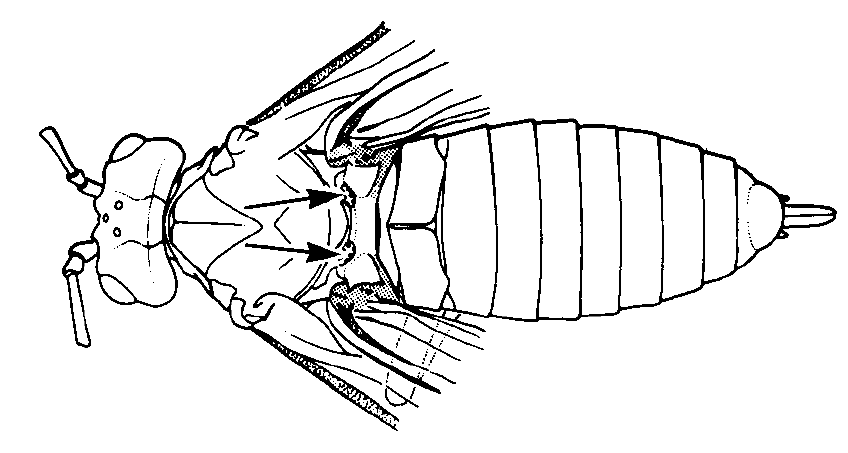
\includegraphics[width=\textwidth]{SymphytaHabitus}
        \caption{Symphytan dorsal habitus \citep[][pg. 42]{goulet1993hymenoptera}}
        \label{fig:symphyt1}
    \end{subfigure}
    \hfill 
    \begin{subfigure}[ht!]{0.45\textwidth}
        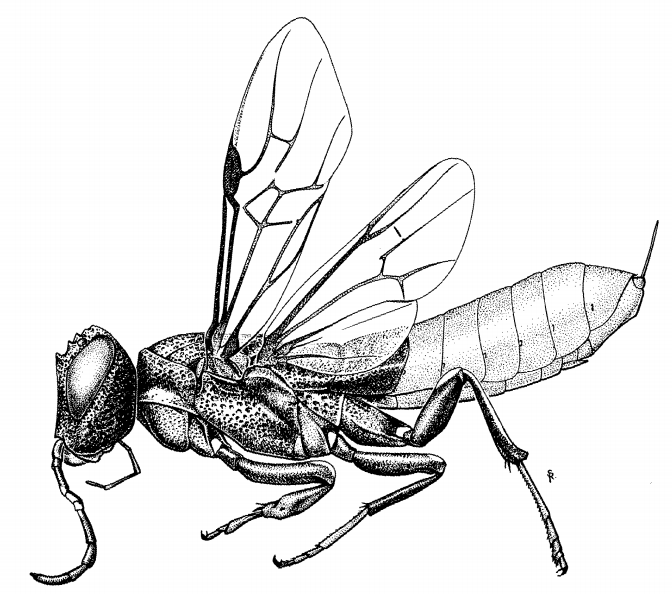
\includegraphics[width=\textwidth]{OrussidHabitus}
        \caption{Orussidae habitus \citep[][Fig. 24]{goulet1993hymenoptera}}
        \label{fig:orussid1}
    \end{subfigure}
    \caption{}\label{fig:symphytans}
\end{figure}

\subsubsection{Xyelidae}
\noindent{}\textit{Diagnostic characters:} Antennae with less than 10 flagellomeres; proximal-most flagellomere much longer than following flagellomeres; maxillary palp leg-like (Figure \ref{fig:xyelids}.\\

\noindent{}\textit{Natural history:} Larvae develop inside pollen-producing cones of pine trees (\textit{Pinus} spp.), while adults can be found very early in the spring, feeding on pine and other tree pollen. The oldest hymenopteran fossils (Triassic) look almost like extant xyelids. There are approximately 50 spp.\\

\noindent\textbf{Question 1:} What is the function of those modified maxillary palps?\vspace{2cm}

\begin{figure}[ht!]
    \centering
    \begin{subfigure}[ht!]{0.4\textwidth}
        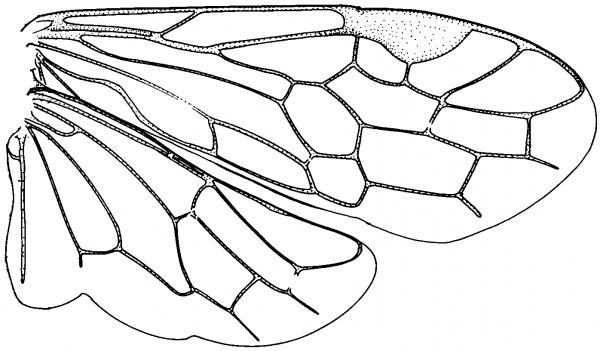
\includegraphics[width=\textwidth]{XyelidWings}
        \caption{Wings \citep[][modified from Fig. 32]{goulet1993hymenoptera}}
        \label{fig:xyelidwings}
    \end{subfigure}
    \hfill 
    \begin{subfigure}[ht!]{0.42\textwidth}
        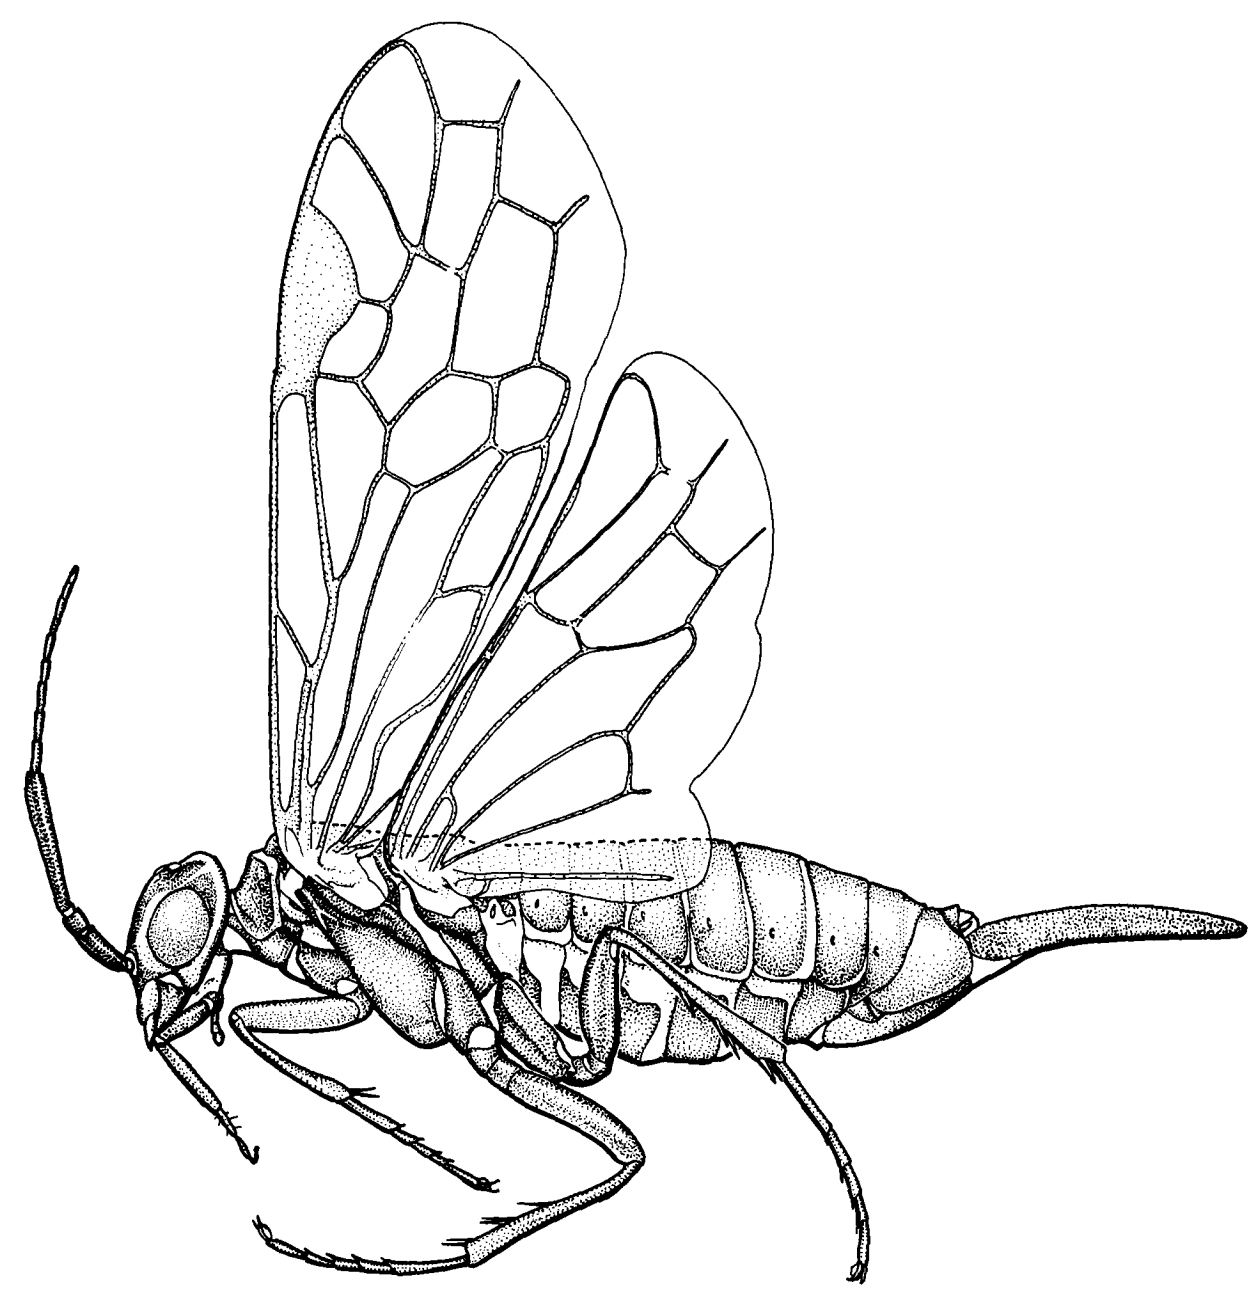
\includegraphics[width=\textwidth]{XyelidHabitus}
        \caption{Habitus \citep[][Fig. 32]{goulet1993hymenoptera}}
        \label{fig:xyelidhead}
    \end{subfigure}
    \caption{Xyelidae}\label{fig:xyelids}
\end{figure}

\subsubsection{Argidae (argid sawflies)}
\noindent{}\textit{Diagnostic characters:} Antenna with 1 flagellomere, sometimes U-shaped (Figure \ref{fig:argid1}); mesonotum not divided by straight transverse groove; fore wing 2r vein absent.\\

\noindent{}\textit{Natural history:} Typically foliage feeders, this taxon is much more diverse in the tropics (\textgreater800 spp.) than in North America ($\sim$70 spp.)\\

\begin{figure}[ht!]
    \centering
    \begin{subfigure}[ht!]{0.11\textwidth}
        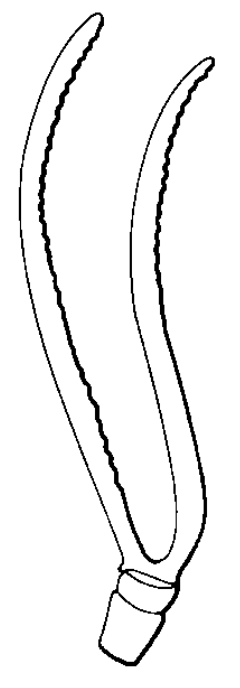
\includegraphics[width=\textwidth]{ArgidAntenna}
        \caption{Antenna}
        \label{fig:argid1}
    \end{subfigure}
    \qquad
    \begin{subfigure}[ht!]{0.45\textwidth}
        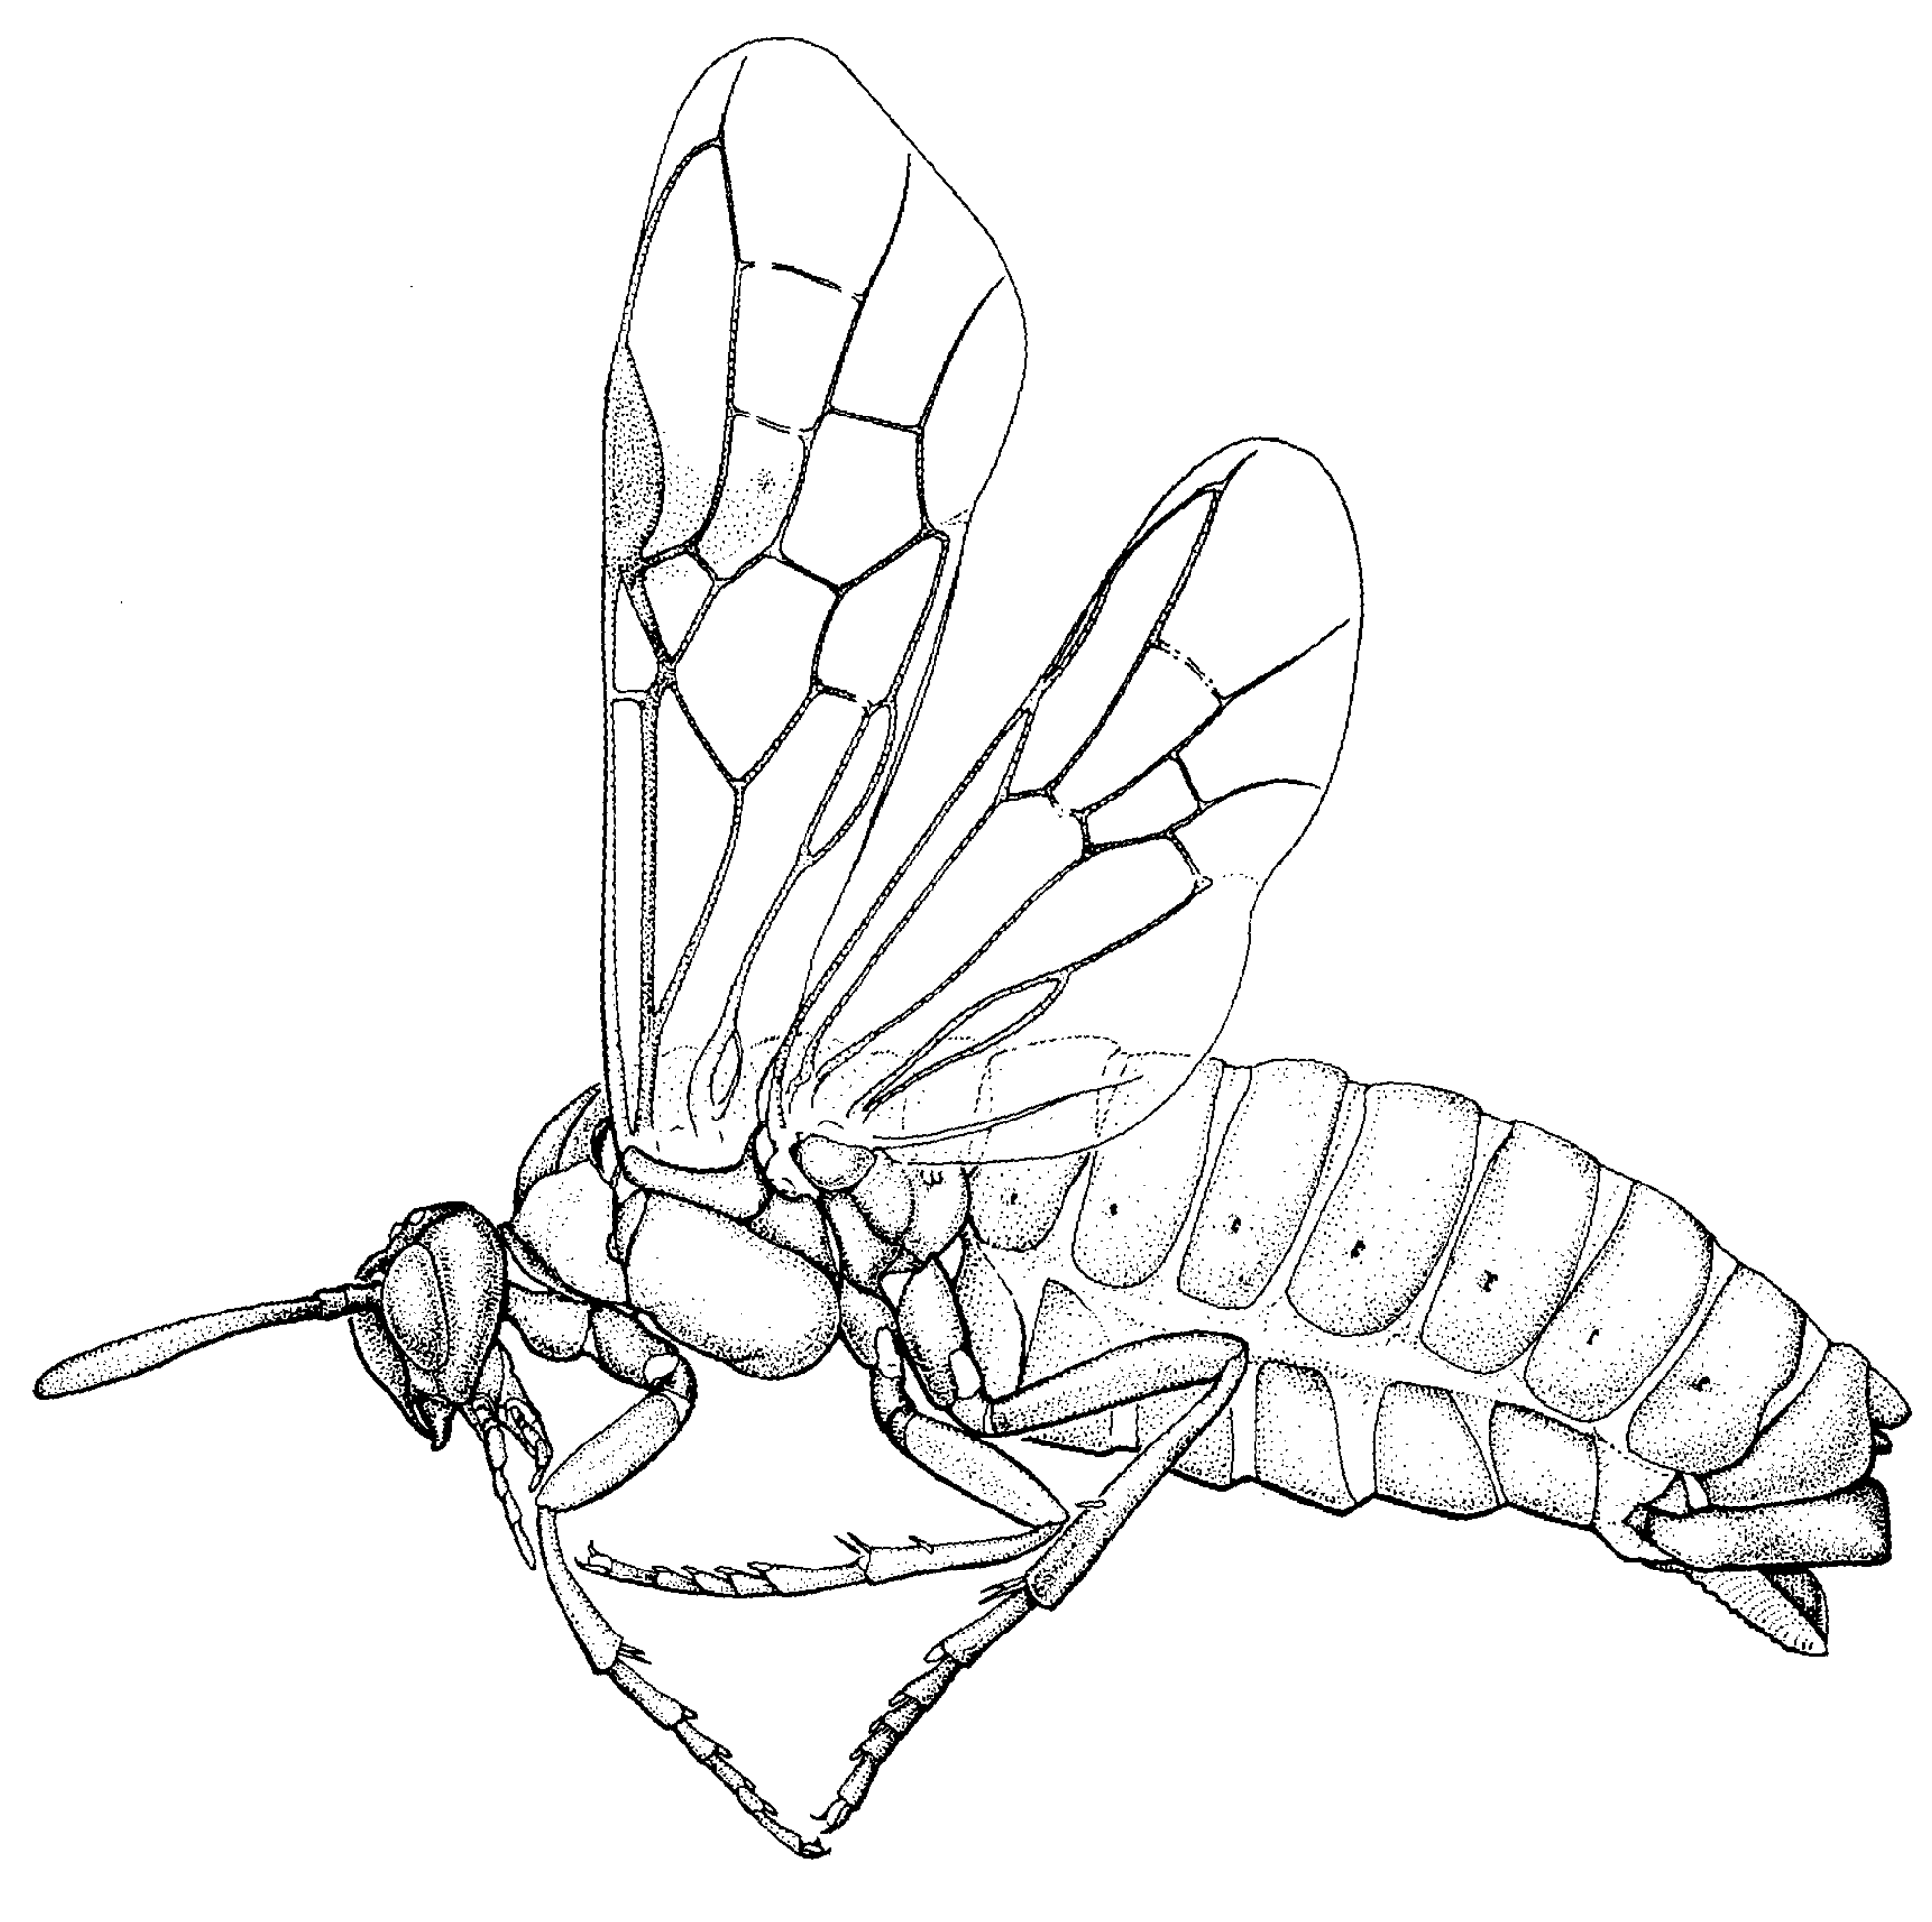
\includegraphics[width=\textwidth]{ArgidHabitus}
        \caption{Habitus}
        \label{fig:argid2}
    \end{subfigure}
    \caption{Argidae \citep[][pg. 106 (a) and Fig. 26 (b)]{goulet1993hymenoptera}}\label{fig:argid}
\end{figure}

\subsubsection{Diprionidae (conifer sawflies)}
\noindent{}\textit{Diagnostic characters:} Antenna with $\sim$20 flagellomeres, comb-like in males and saw-like in females; fore wing with less than 2 marginal cells; abdominal tergum 1 separated from metapleuron in both sexes.\\

\noindent{}\textit{Natural history:} Larvae develop as folivores on pines. Some species are considered pests. Larvae often feed gregariously, regurgitating pine resin when disturbed. Almost 100 species have been described.\\

\begin{figure}[ht!]
    \centering
    \begin{subfigure}[ht!]{0.14\textwidth}
        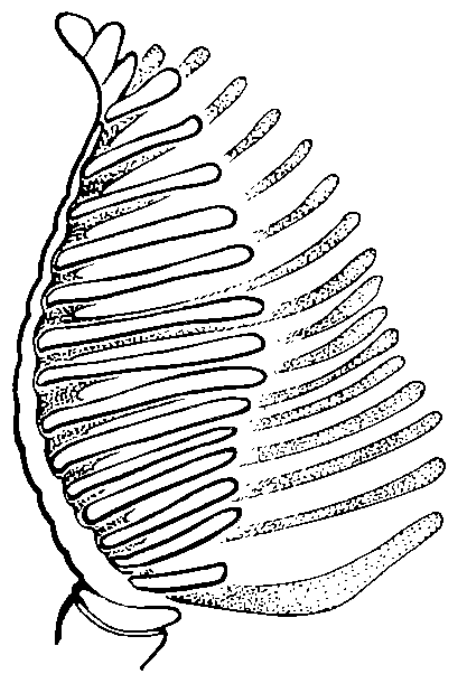
\includegraphics[width=\textwidth]{DiprionidAntenna}
        \caption{Male antenna}
        \label{fig:diprionid1}
    \end{subfigure}
    \qquad
    \begin{subfigure}[ht!]{0.42\textwidth}
        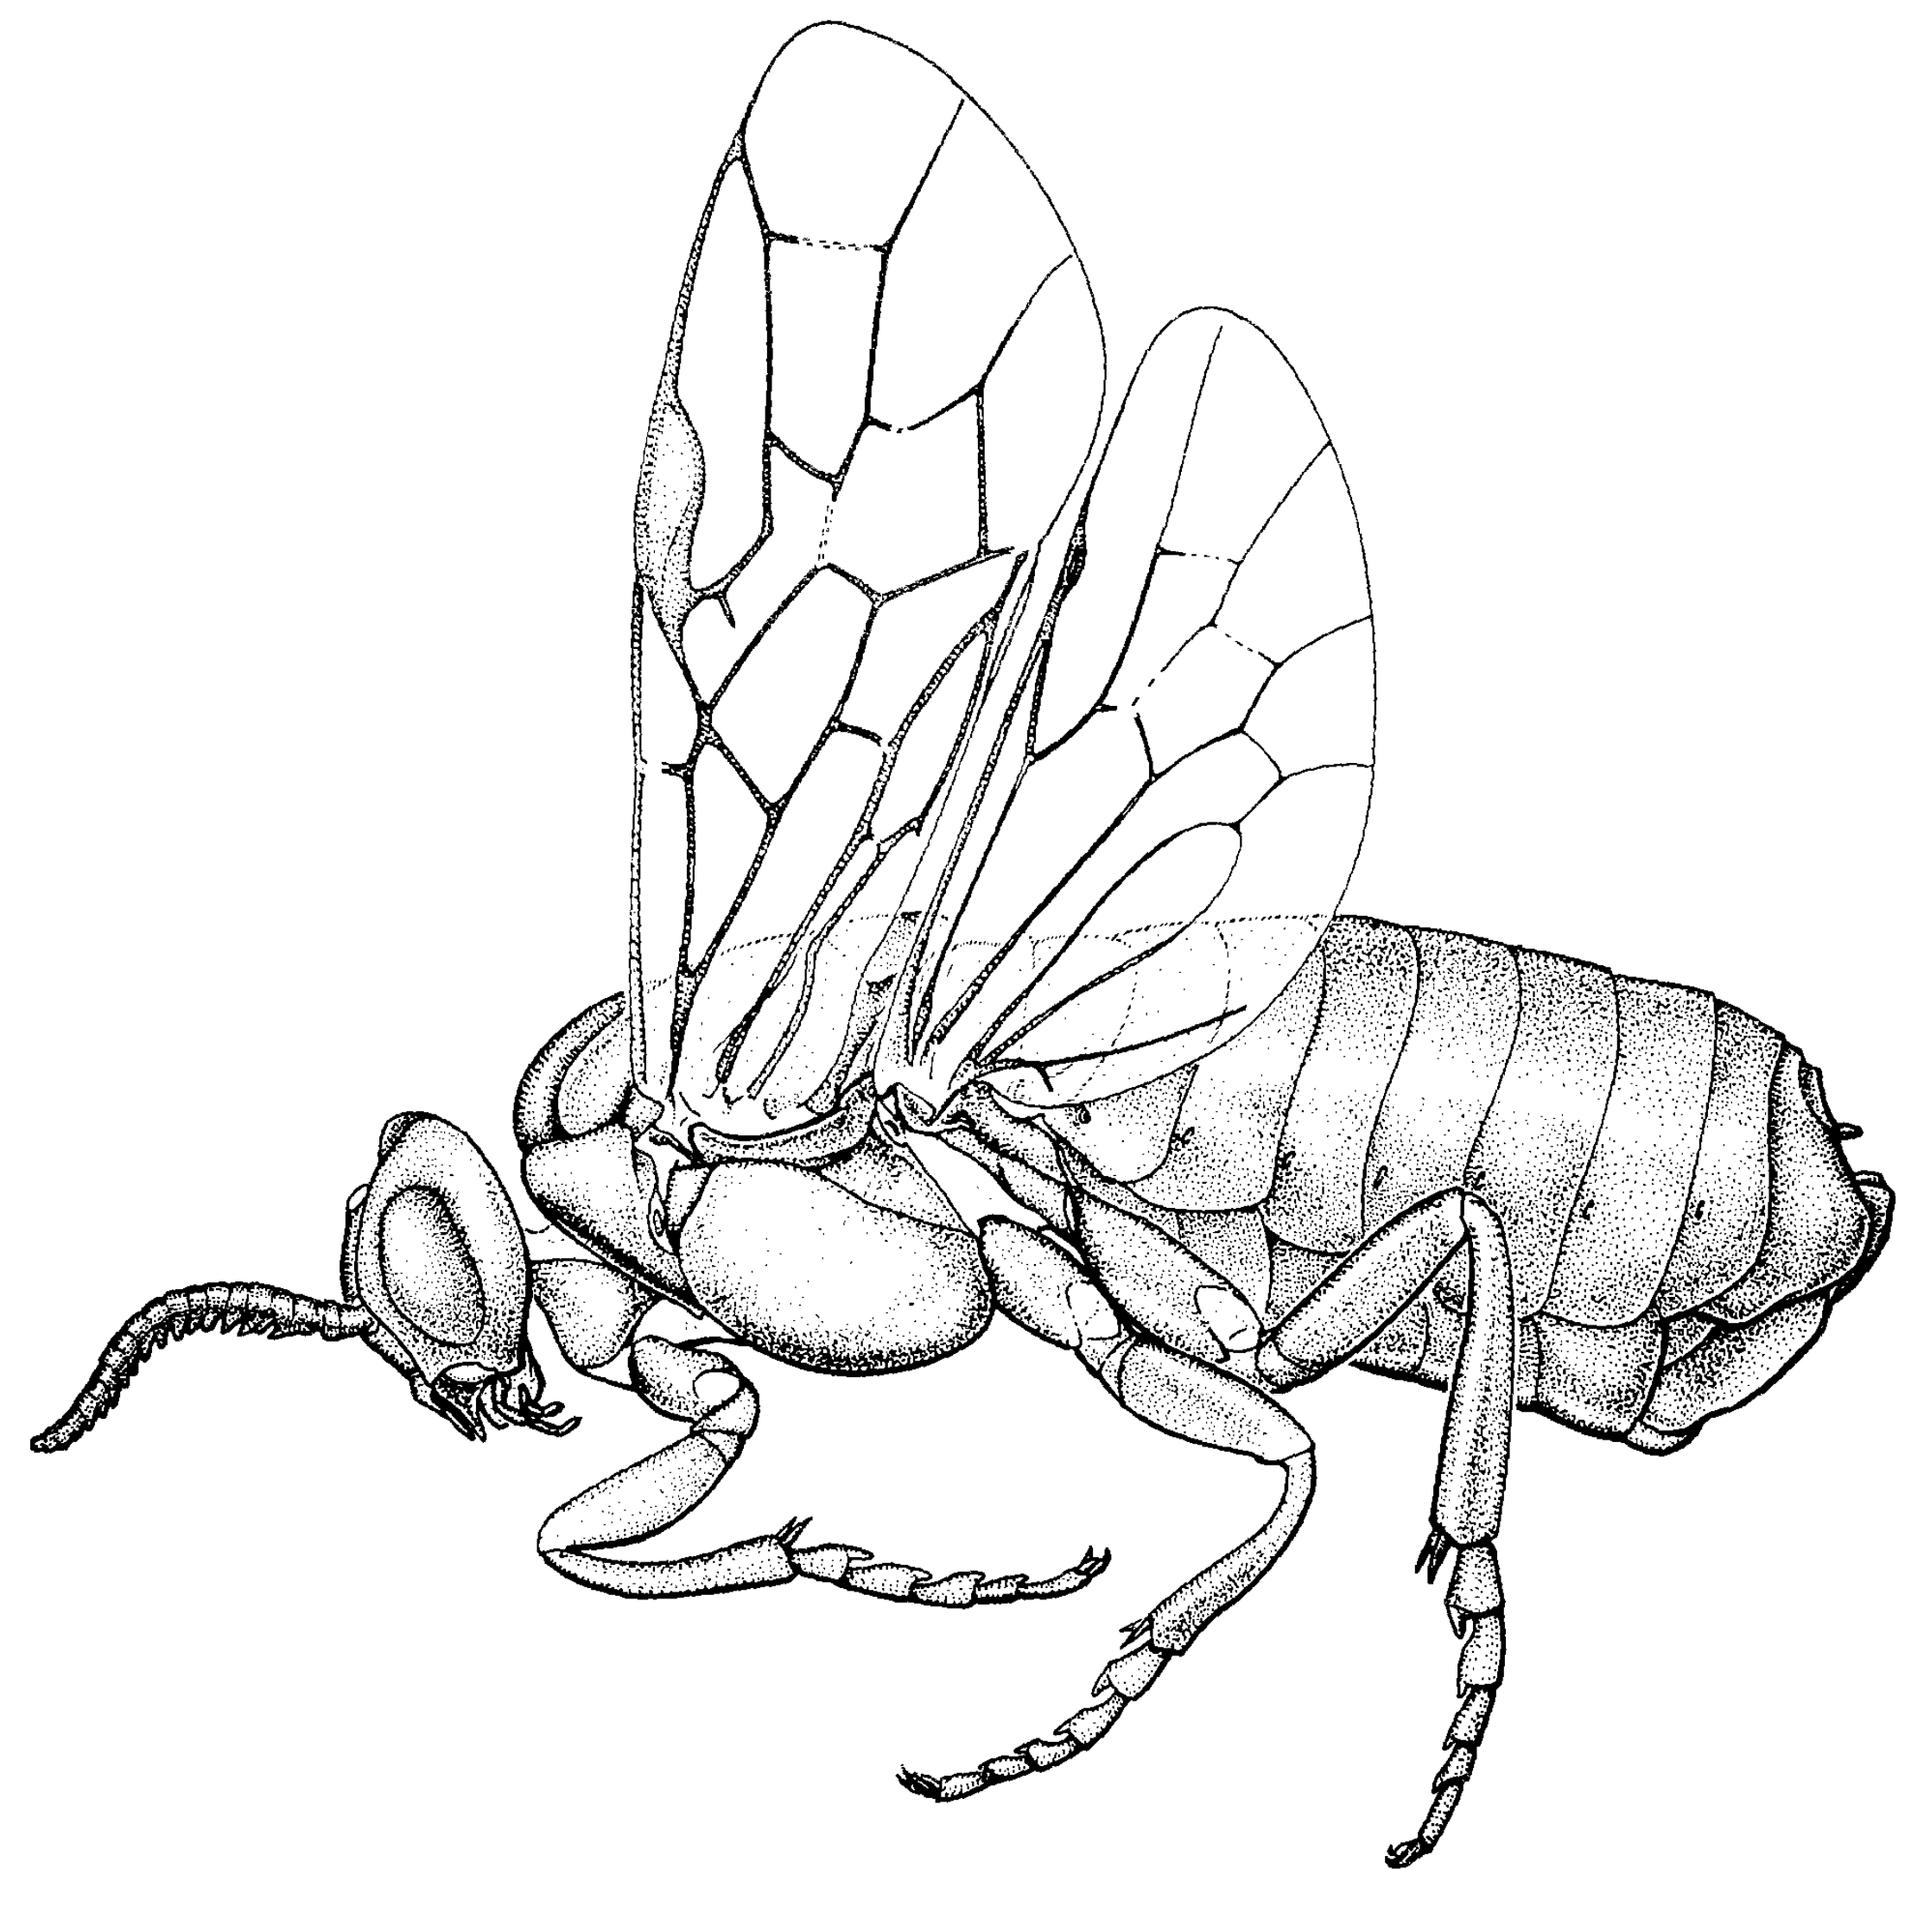
\includegraphics[width=\textwidth]{DiprionidHabitus}
        \caption{Habitus, male (left) and female (right)}
        \label{fig:diprionid2}
    \end{subfigure}
    \caption{Diprionidae \citep[][pg. 108 (a) and Fig. 29 (b)]{goulet1993hymenoptera}}\label{fig:diprion}
\end{figure}

\subsubsection{Tenthredinidae (common sawflies)}
\noindent{}\textit{Diagnostic characters:} Antenna with 3--7 flagellomeres (Figure \ref{fig:tenthred1}); abdominal tergum 1 clearly separated from metapleuron.\\

\noindent{}\textit{Natural history:} Larvae are diversely phytophagous, developing as folivores, borers, gallers, and even leaf miners. There are more than 7,000 described spp.\\

\begin{figure}[ht!]
  \centering
    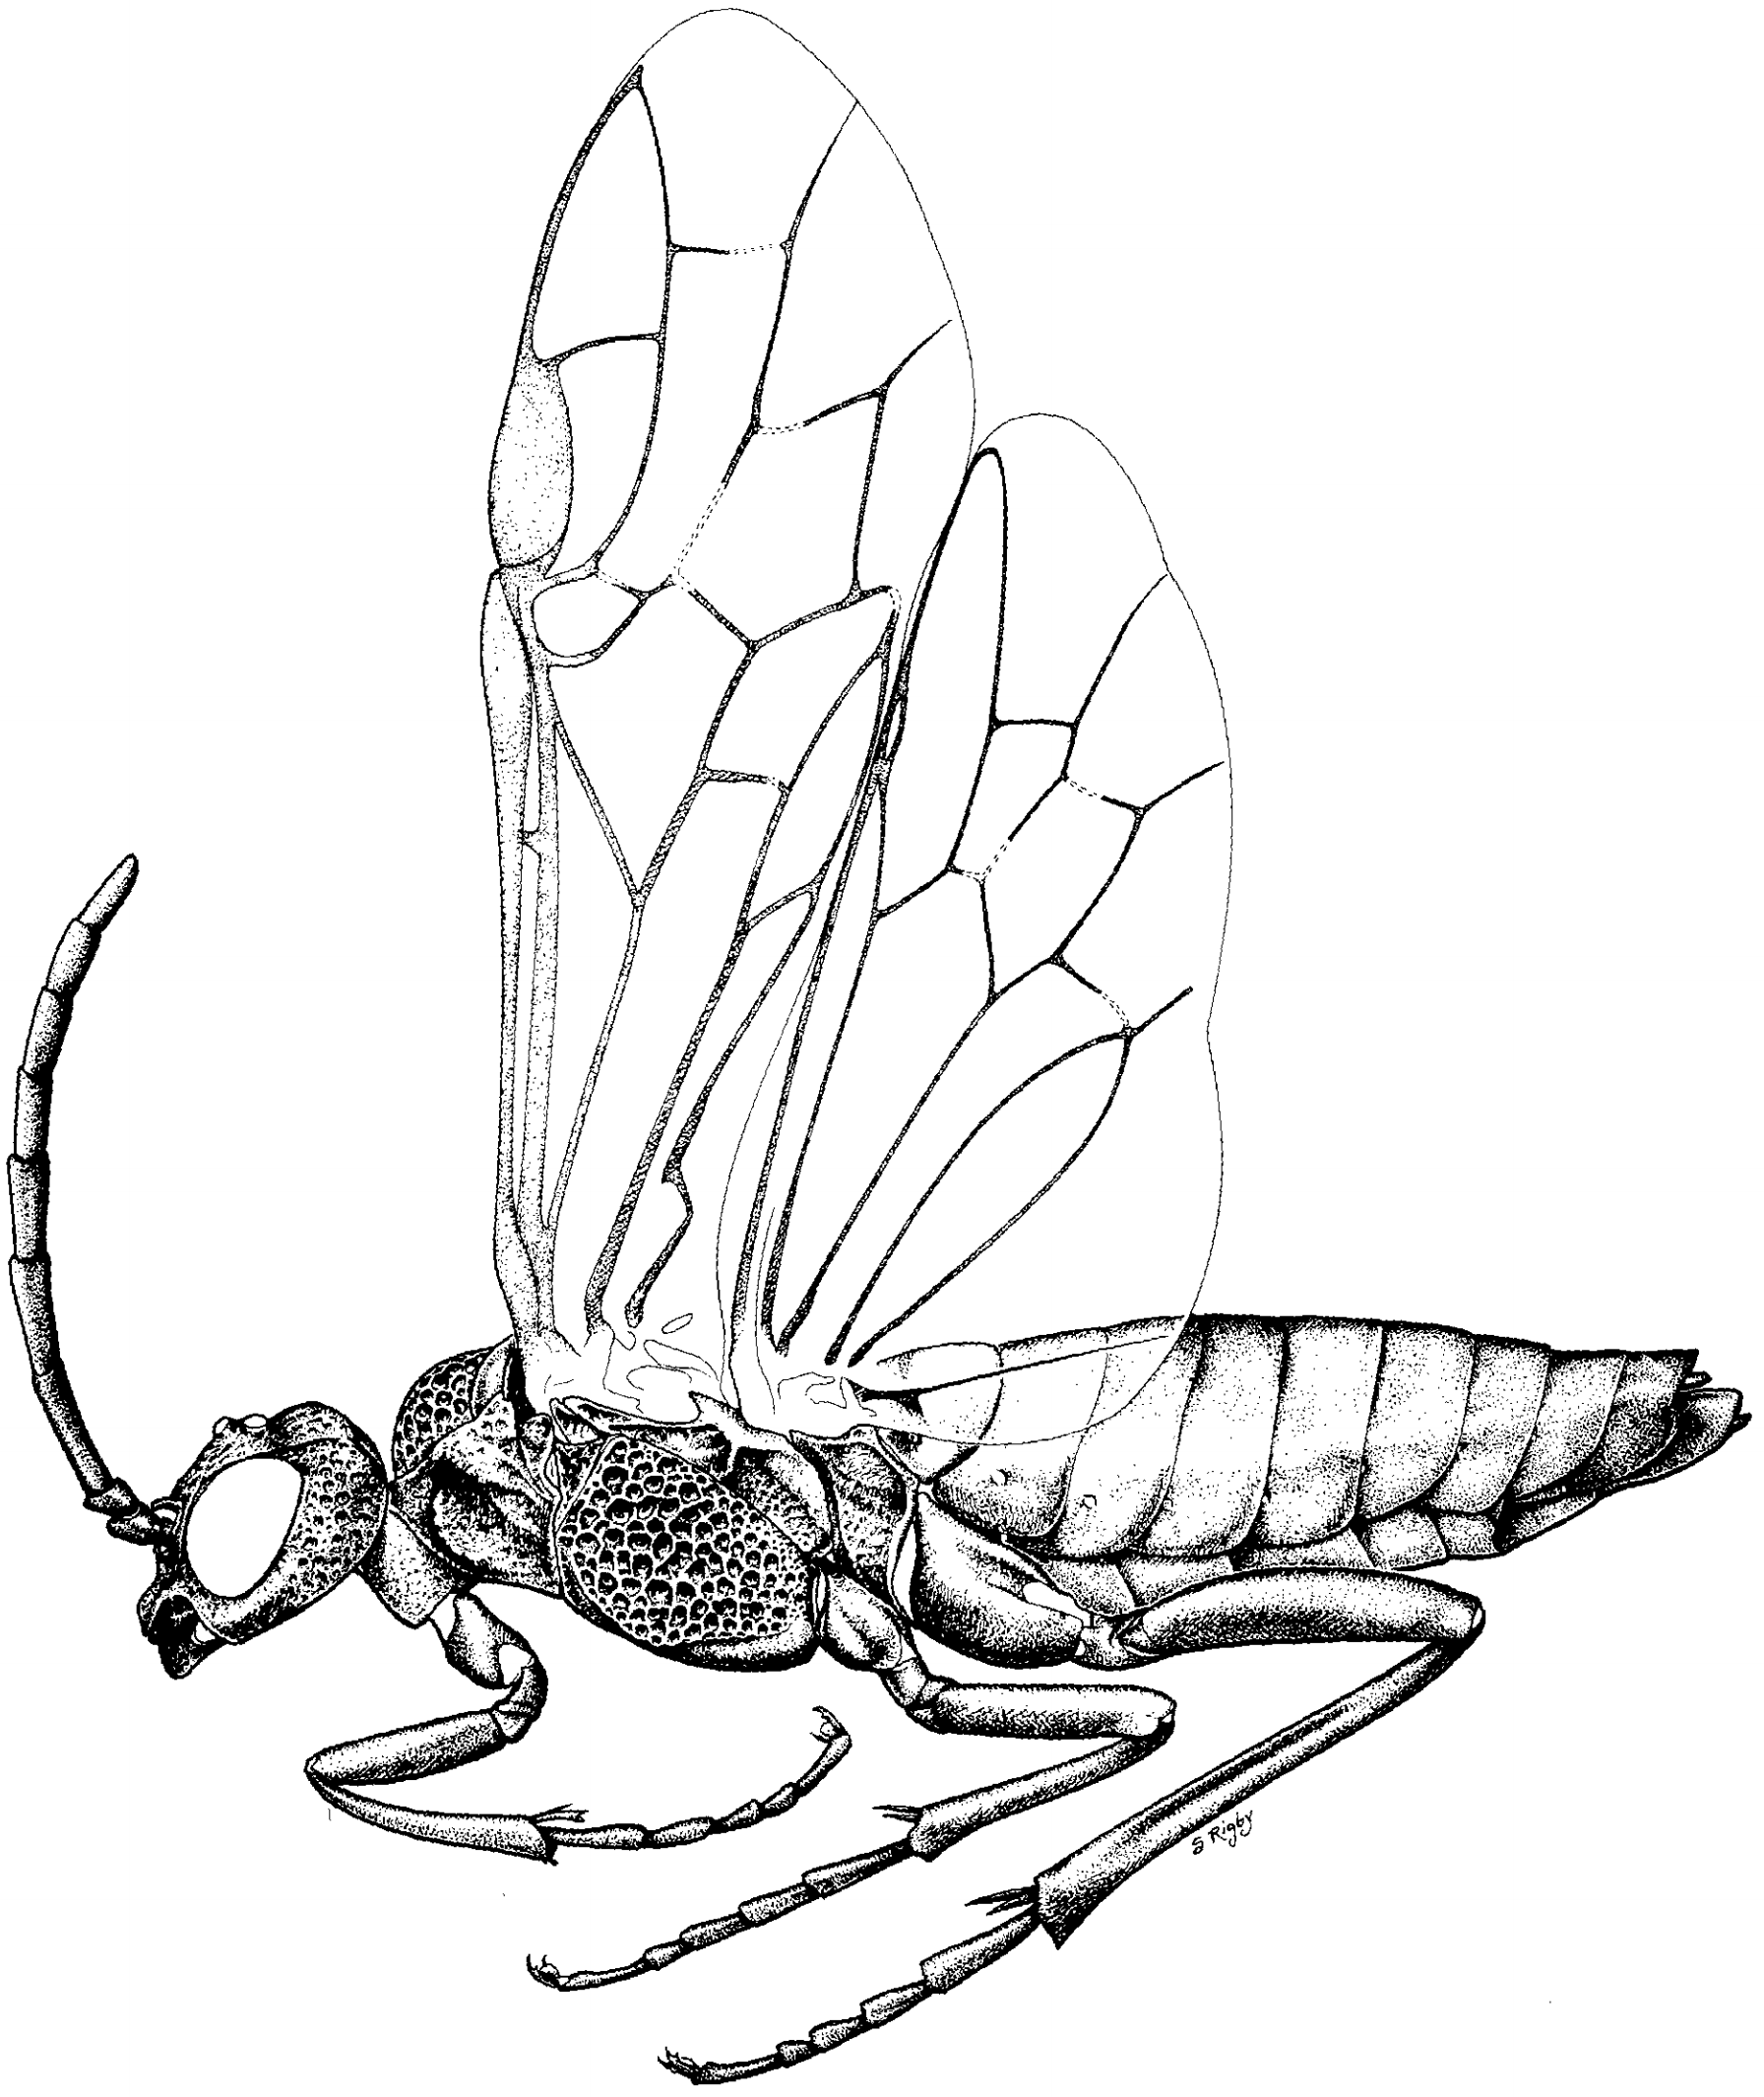
\includegraphics[width=0.4\textwidth]{TenthredinidHabitus}
  \caption{Tenthredinidae, lateral habitus \citep[][Fig. 31]{goulet1993hymenoptera}}
  \label{fig:tenthred1}
\end{figure}

\noindent{}The next two families represent a transition in life history, from larvae feeding mostly on leaves to larvae feeding inside wood. \\

\noindent\textbf{Question 2:} Can you see evidence of this transition in the external morphology of these hymenopterans? Compare these next two taxa to Tenthredinidae or Argidae, for example, and describe or illustrate a few differences. What is the function of the transcutal articulation?\vspace{3cm}

\subsubsection{Siricidae (horntails)}
\noindent{}\textit{Diagnostic characters:} Antenna with \textgreater{}20 flagellomeres; pronotum with a large dorsal (horizontal) surface (Figure \ref{fig:siricid1}); fore tibia with one apical spur; posterior-most tergum in females and sternum in males with apical projection (Figure \ref{fig:siricid2})\\

\noindent{}\textit{Natural history:} There are $\sim$150 described species. Female siricids have pockets (``mycangia''; we'll see this word again when we cover Coleoptera) at the base of their ovipositors that contain fungi. \\

\noindent\textbf{Question 3:} What do you think is the role of the symbiotic fungi found in siricids?\vspace{1.5cm}

\begin{figure}[ht!]
    \centering
    \begin{subfigure}[ht!]{0.36\textwidth}
        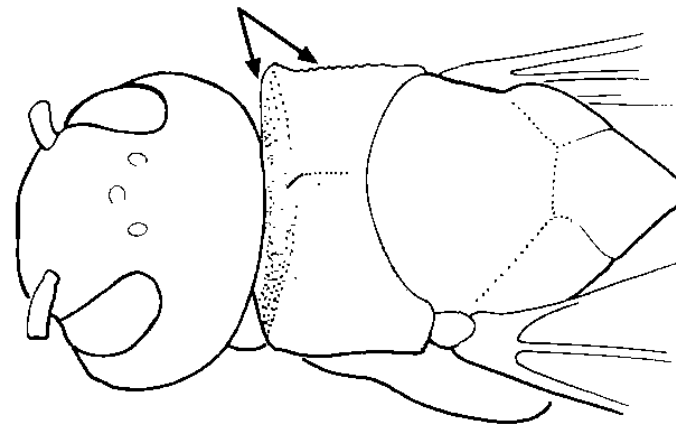
\includegraphics[width=\textwidth]{SiricidPronotum}
        \caption{Siricidae, dorsal head and thorax \citep[][pg. 70]{goulet1993hymenoptera}}
        \label{fig:siricid1}
    \end{subfigure}
    \hfill
    \begin{subfigure}[ht!]{0.42\textwidth}
        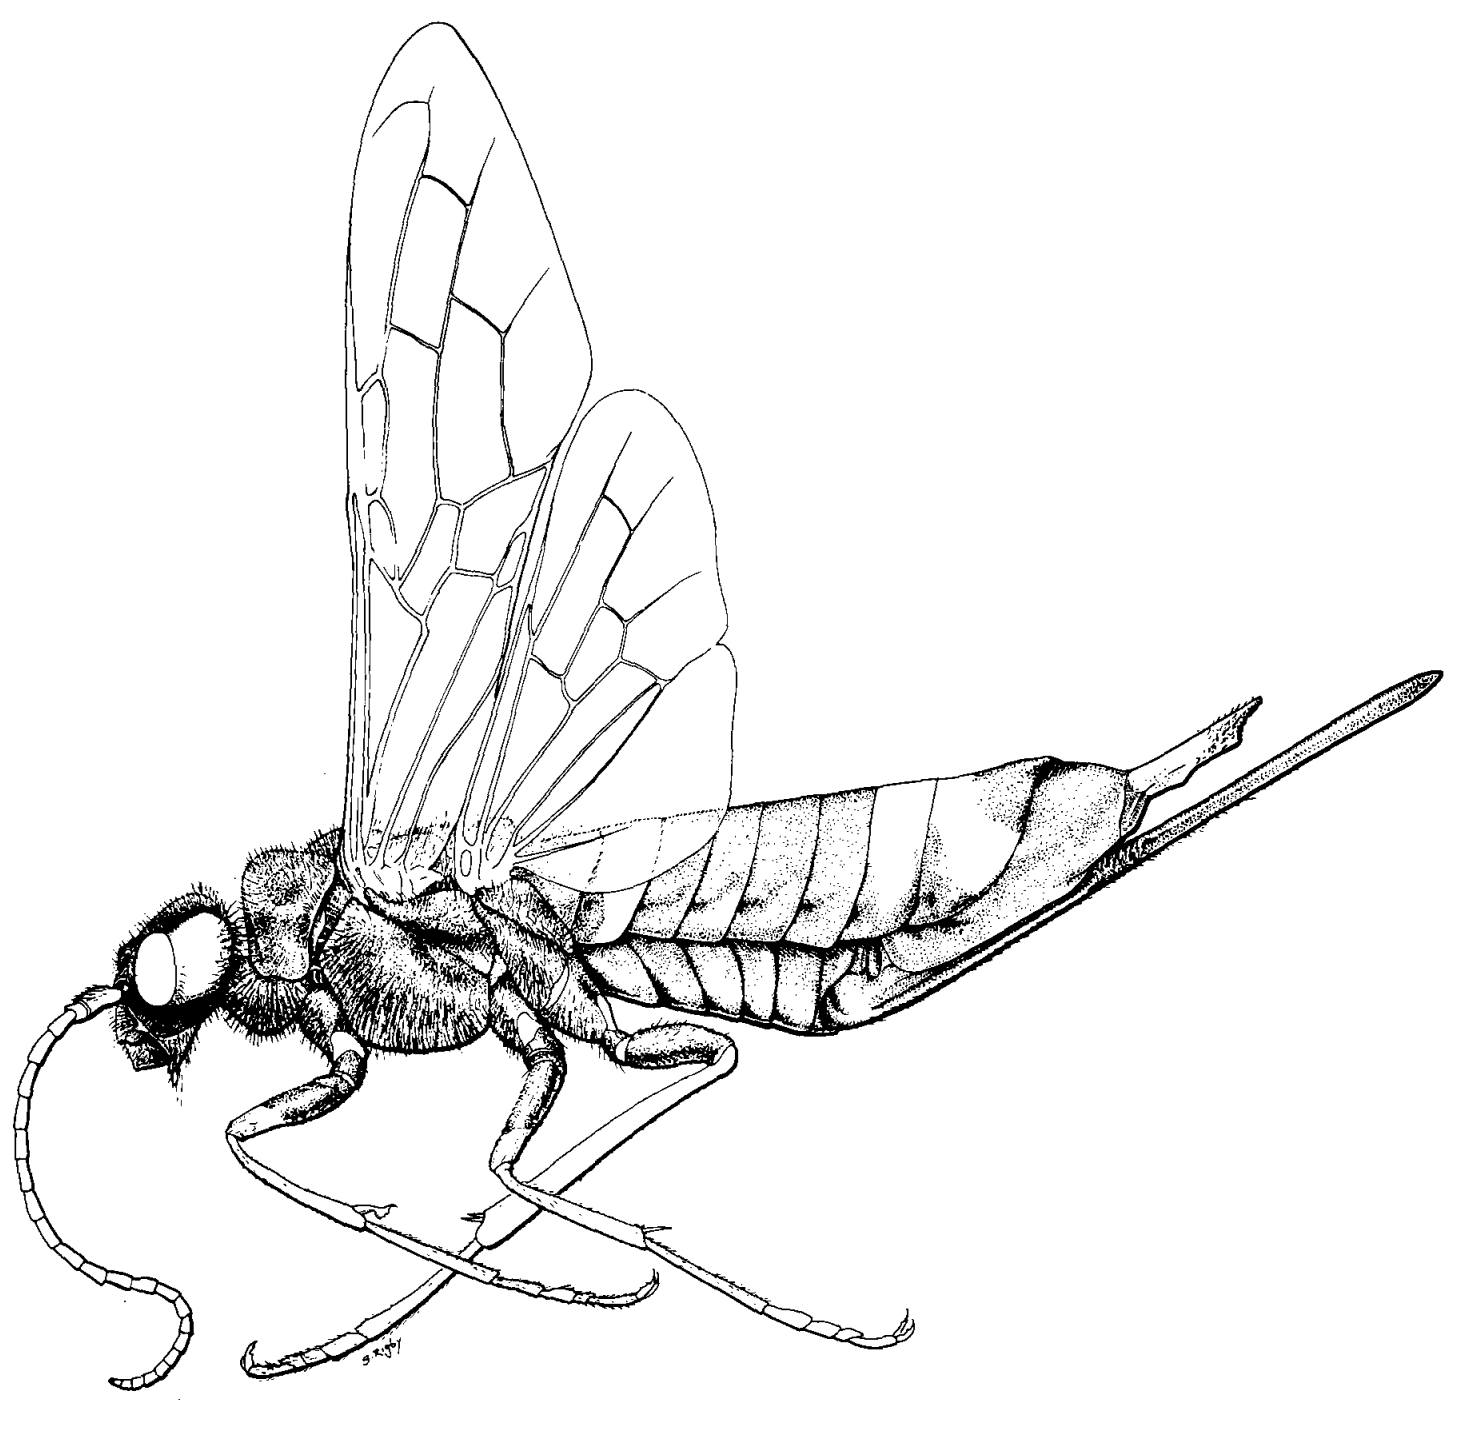
\includegraphics[width=\textwidth]{SiricidHabitus}
        \caption{Habitus \citep[][Fig. 25]{goulet1993hymenoptera}}
        \label{fig:siricid2}
    \end{subfigure}
    \caption{Siricidae}\label{fig:siricids}
\end{figure}

\subsection{Apocrita}
The remaining hymenopterans comprise the megadiverse Apocrita, a lineage characterized in part, at least ancestrally, by developing as parasitoids of other insects. In dorsal view, the body has a distinct constriction near its middle (\textit{i.e.}, ``wasp waist'' present); note that the middle tagma is referred to as the ``mesosoma'' and the posteriormost tagma is the ``metasoma''. \\

\subsubsection{Evaniidae (ensign or hatchet wasps)}
\noindent{}\textit{Diagnostic characters:} Antenna with 13 antennomeres (one neotropical genus has 10); pterostigma relatively small; mesosoma relatively stout; hind wing with jugal lobe; metasoma arising dorsally on mesosoma, distance between propodeal foramen and metacoxal cavity much larger than width of either opening; metasoma hatchet-shaped; petiole tubular.\\

\noindent{}\textit{Natural history:} These wasps develop as solitary predators of cockroach eggs, inside the ootheca. Approximately 550 species have been described, but only a handful occur in North America.\\

\begin{figure}[ht!]
  \centering
\begin{subfigure}[ht!]{0.45\textwidth}
    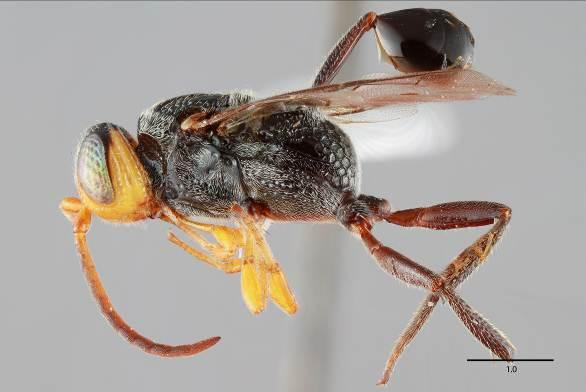
\includegraphics[width=\textwidth]{EvaniidHabitus}
  \caption{Lateral habitus Photo (CC BY 2.0) by \cite{MullinsEtAl2012}}
  \label{fig:evaniid1}
\end{subfigure}
    \hfill
\begin{subfigure}[ht!]{0.45\textwidth}
    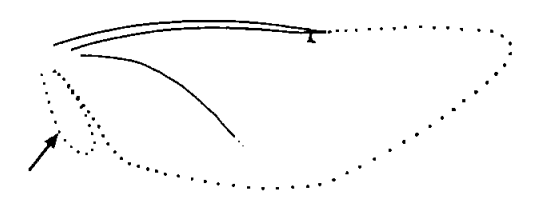
\includegraphics[width=\textwidth]{EvaniidWing}
  \caption{Hind wing \citep[][pg. 510]{goulet1993hymenoptera}}
  \label{fig:evaniid2}
\end{subfigure}
    \caption{Evaniidae}
    \label{fig:evaniid}
\end{figure}

\subsubsection{Megaspilidae}
\noindent{}\textit{Diagnostic characters:} Antenna with 12 antennomeres (Figure \ref{fig:megaspilid2}); fore wing with no cells enclosed by tubular veins (Figure \ref{fig:megaspilid1})and only 1 proximal tubular vein on anterior margin; pterostigma distinct; protibia with two apical spurs; pronotum adjacent to tegula in lateral view (compare to Chalcidoidea).\\

\noindent{}\textit{Natural history:} Parasitoids of many kinds of insects, including other parasitoid Hymenoptera (\textit{i.e.}, some megaspilids are hyperparasitoids). These wasps are relatively easy to collect, and there are just over 300 species known worldwide.\\

\begin{figure}[ht!]
  \centering
\begin{subfigure}[ht!]{0.45\textwidth}
    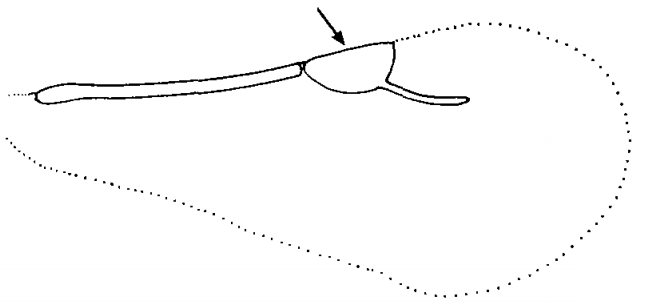
\includegraphics[width=\textwidth]{MegaspilidWing}
  \caption{Fore wing \citep[][pg. 566]{goulet1993hymenoptera}}
  \label{fig:megaspilid1}
\end{subfigure}
    \hfill
\begin{subfigure}[ht!]{0.45\textwidth}
    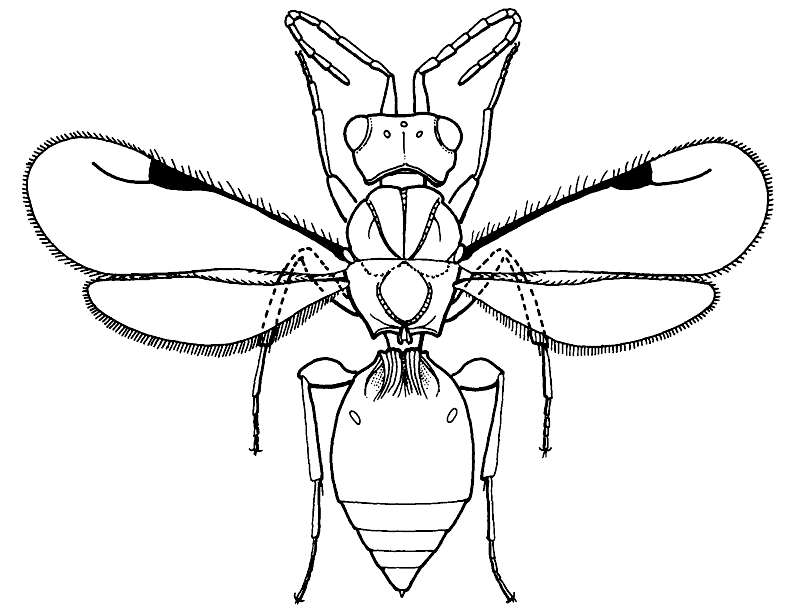
\includegraphics[width=\textwidth]{MegaspilidHabitus}
  \caption{Dorsal habitus \citep[][Fig. 209]{goulet1993hymenoptera}}
  \label{fig:megaspilid2}
\end{subfigure}
    \caption{Megaspilidae}\label{fig:megaspilid}
\end{figure}

\subsubsection{Braconidae}
\noindent{}\textit{Diagnostic characters:} Antenna usually with 16 or more antennomeres (Figure \ref{fig:braconid1}); fore wing C + Sc + R fused (\textit{i.e.}, anterior margin of wing with relatively thick wing vein); pterostigma usually present; one recurrent vein or none (Figure \ref{fig:braconid2} arrow); no ``horse head'' cell (compare with Ichneumonidae); first and second metasomal segments often fused and immobile dorsally.\\

\noindent{}\textit{Natural history:} These parasitoid wasps are extraordinarily diverse, with almost 20,000 described species. Many of them, especially the subfamily Microgastrinae, coevolved with viruses (polydnaviruses), which help them overcome the ho hosts' immune response.\\

\begin{figure}[ht!]
    \centering
    \begin{subfigure}[ht!]{0.55\textwidth}
        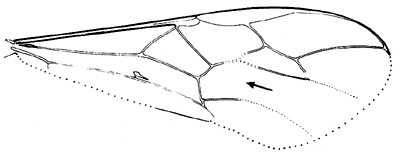
\includegraphics[width=\textwidth]{BraconidWing}
        \caption{Fore wing \citep[][pg. 359]{goulet1993hymenoptera}}
        \label{fig:braconid1}
    \end{subfigure}
    \hfill
    \begin{subfigure}[ht!]{0.34\textwidth}
        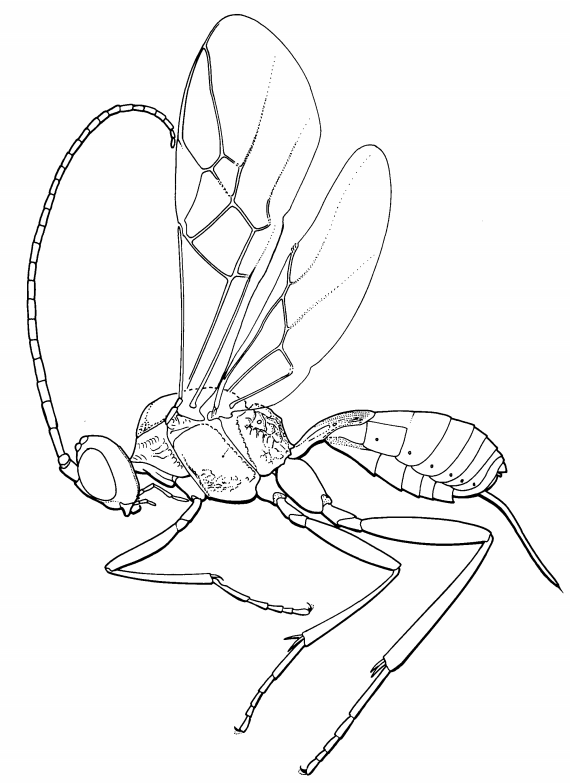
\includegraphics[width=\textwidth]{BraconidHabitus}
        \caption{Lateral habitus \citep[][Fig. 138]{goulet1993hymenoptera}}
        \label{fig:braconid2}
    \end{subfigure}
    \caption{Braconidae}\label{fig:braconids}
\end{figure}

\subsubsection{Ichneumonidae (ichneumon wasps)}
\noindent{}\textit{Diagnostic characters:} Antenna usually with 16 or more antennomeres; fore wing C + Sc + R fused (\textit{i.e.}, anterior margin of wing with relatively thick wing vein); pterostigma usually present; two recurrent veins present (Figure \ref{fig:ichneumonid1} arrow); ``horse head cell'' present (often not quite horse-like); first and second metasomal segments not fused.\\

\noindent{}\textit{Natural history:} One of the most diverse families of insects, with at least 24,000 named species and many, many more remaining to be described. Like their sister family, Braconidae, some species inject polydnaviruses into the hosts, along with the egg(s), to combat the hosts' immune responses. These wasps are parasitoids of many kinds of arthropods but mostly other insects.\\

\begin{figure}[ht!]
    \centering
    \begin{subfigure}[ht!]{0.5\textwidth}
        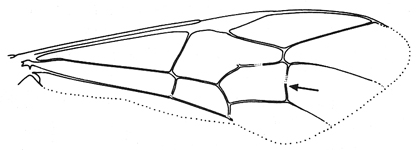
\includegraphics[width=\textwidth]{IchneumonidWing}
        \caption{Fore wing \citep[][pg. 359]{goulet1993hymenoptera}}
        \label{fig:ichneumonid1}
    \end{subfigure}
    \hfill
    \begin{subfigure}[ht!]{0.4\textwidth}
        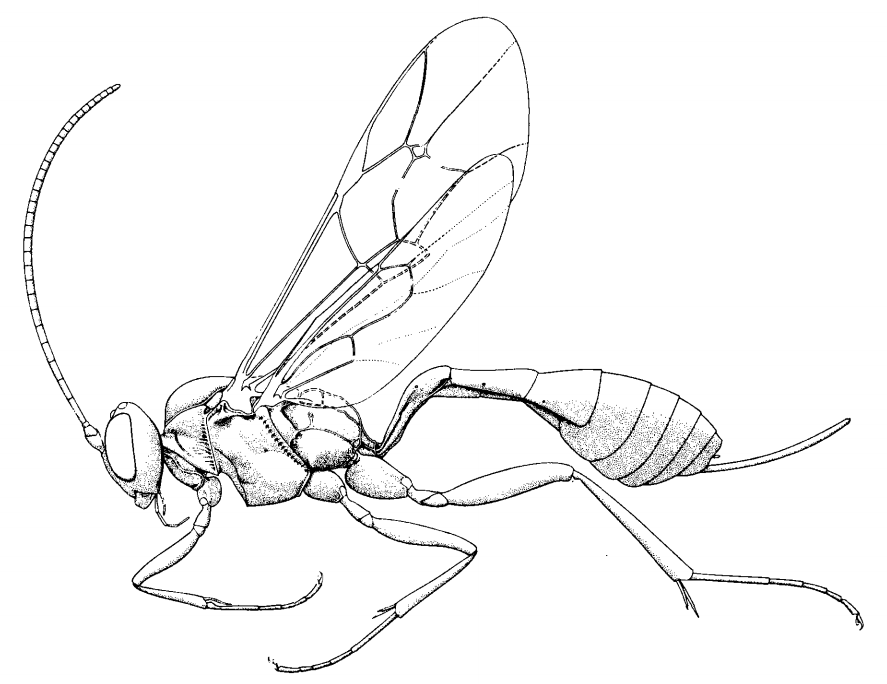
\includegraphics[width=\textwidth]{IchneumonidHabitus}
        \caption{Lateral habitus \citep[][Fig. 159]{goulet1993hymenoptera}}
        \label{fig:ichneumonid2}
    \end{subfigure}
    \caption{Ichneumonidae}\label{fig:ichneumonids}
\end{figure}

\subsubsection{Diapriidae}
\noindent{}\textit{Diagnostic characters:} Antenna elbowed; antennal shelf present, articulation dorsally distant from clypeus; antenna with 11--15 antennomeres; fore wing venation variable (sometimes lacking wing cells); usually black or brown, often shiny and smooth in parts; petiole tubular.\\

\noindent{}\textit{Natural history:} Approximately 2,500 species have been described from around the world. These wasps are very frequently collected in yellow pans and leaf litter samples, and most species are understood to be parasitoids of larval dipterans.\\

\begin{figure}[ht!]
  \centering
    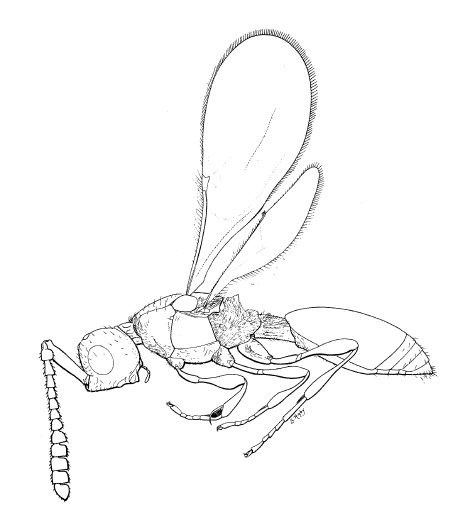
\includegraphics[width=0.45\textwidth]{DiapriidHabitus}
  \caption{Diapriidae habitus \citep[][Fig. 206]{goulet1993hymenoptera}}
  \label{fig:diapriid1}
\end{figure}

\subsubsection{Pelecinidae}
\noindent{}\textit{Diagnostic characters:} relatively large (20--70 mm long); fore wing with one cell enclosed by tubular veins; petiole tubular, female abdominal segments elongate, tubular (Figure \ref{fig:pelecinid1}).\\

\noindent{}\textit{Natural history:} There is only one extant species, whose distribution spans from Canada to Argentina. Females use their extended metasomas to probe soil for hosts, which are larval scarab beetles (\textit{Phyllophaga} spp.)\\

\begin{figure}[ht!]
  \centering
    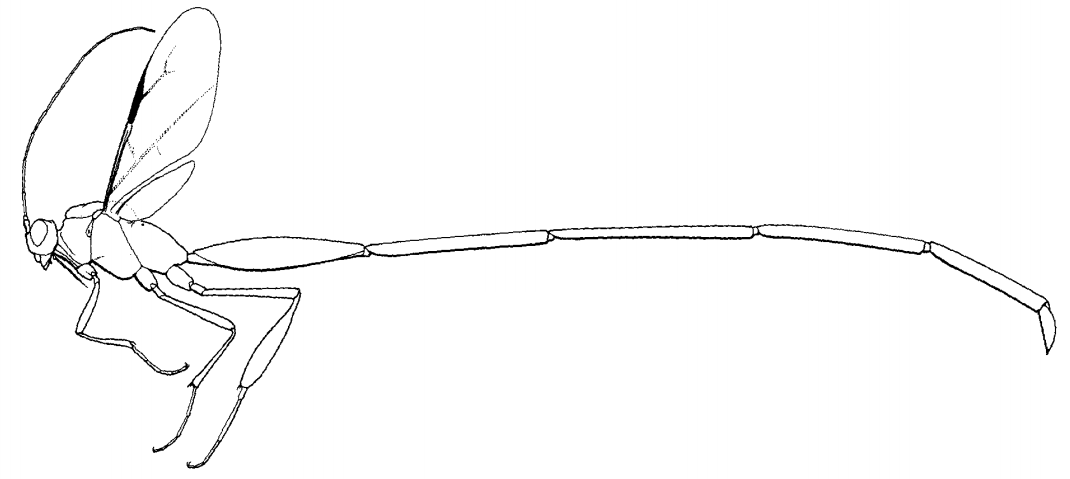
\includegraphics[width=0.75\textwidth]{PelecinidHabitus}
  \caption{Pelecinidae, female habitus. \citep[][Fig. 198]{goulet1993hymenoptera}}
  \label{fig:pelecinid1}
\end{figure}

\subsubsection{Scelionidae}
\noindent{}\textit{Diagnostic characters:} Antenna elbowed; antennal shelf absent; antennal sockets usually close to clypeus; fore wing with 3 veins, pterostigma absent (Figure \ref{fig:scelionid1}); fore wing without proximal tubular vein on anterior margin; antenna usually with 11--12 antennomeres; small to very small, usually black or brown; pronotum adjacent to tegula; petiole not tubular; abdomen often flat, with sharp lateral edges.\\

\noindent{}\textit{Natural history:} More than 3,000 species have been described from around the world. These wasps are parasitoids of insect eggs, and several species have been recruited for biocontrol. \\

\noindent\textbf{Question 4:} What do you notice about scelionid body shapes? What do you think is their biological significance?\\

\begin{figure}[ht!]
  \centering
\begin{subfigure}[ht!]{0.45\textwidth}
    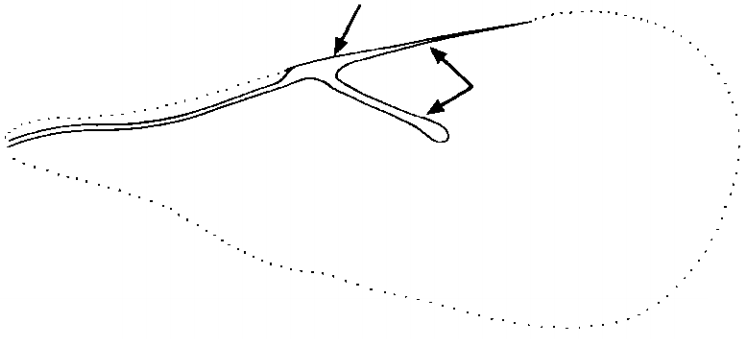
\includegraphics[width=\textwidth]{ScelionidWing}
  \caption{Fore wing \citep[][pg. 560]{goulet1993hymenoptera}}
  \label{fig:scelionid1}
\end{subfigure}
    \hfill
\begin{subfigure}[ht!]{0.45\textwidth}
    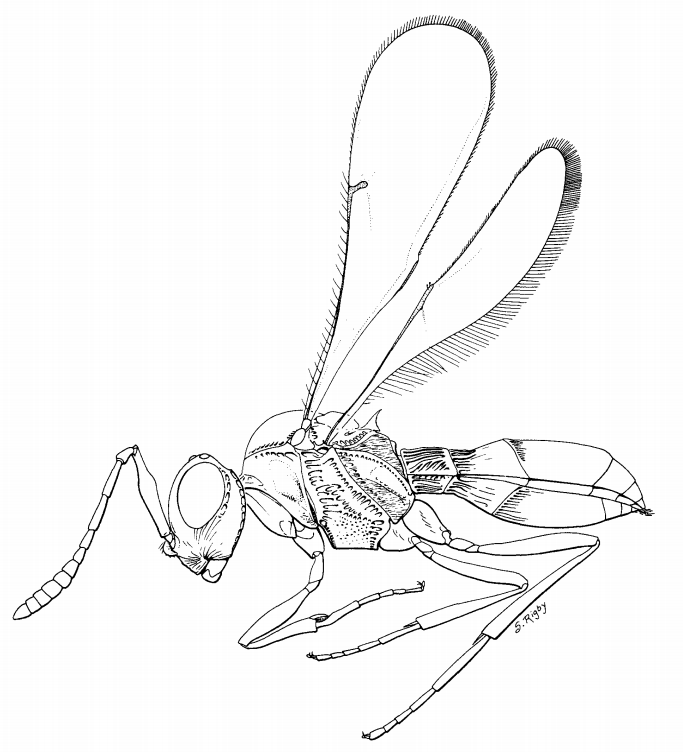
\includegraphics[width=\textwidth]{ScelionidHabitus}
  \caption{Lateral habitus \citep[][Fig. 207]{goulet1993hymenoptera}}
  \label{fig:scelionid2}
\end{subfigure}
    \caption{Scelionidae}\label{fig:scelionids}
\end{figure}

\noindent{}The next two families we cover are classified in Cynipoidea, which share the following characteristics:
\begin{itemize}
\item distinctive wing venation: no proximal vein along anterior margin, with well developed marginal cell (R1), no pterostigma
\item antenna with 11--16 antennomeres, not elbowed (\textit{i.e}., not geniculate)
\item abdomen laterally flattened
\end{itemize}

\subsubsection{Figitidae}
\noindent{}\textit{Diagnostic characters:} Fore wing with cell RI 3--4 times as long as wide; hind leg with tarsomere 1 not longer than remaining tarsomeres combined; petiole of metasoma usually elongate, longer than wide; scutellum usually elaborate, with keel or oval elevation; if scutellum not elaborate, then 3 abdominal tergites visible or head wider than mesosoma.\\

\noindent{}\textit{Natural history:} There are $\sim$1,400 described species, the vast majority of which are parasitoids of Diptera larvae. Some species are hyperparasitoids on Sternorrhyncha. \\

\begin{figure}[ht!]
  \centering
\begin{subfigure}[ht!]{0.45\textwidth}
    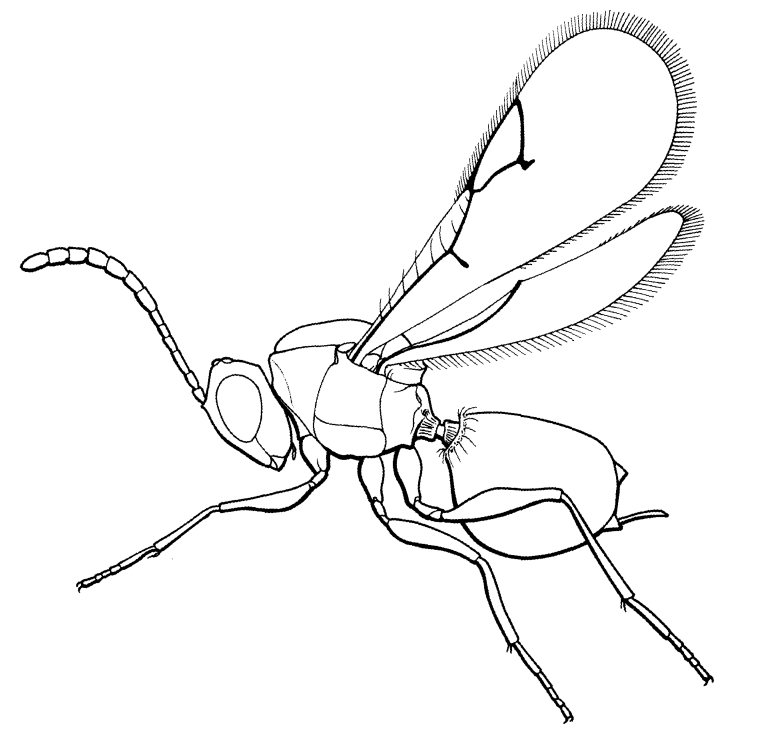
\includegraphics[width=\textwidth]{FigitidHabitus}
  \caption{Figitidae habitus \citep[][Fig. 195]{goulet1993hymenoptera}}
  \label{fig:figid1}
\end{subfigure}
    \hfill
\begin{subfigure}[ht!]{0.42\textwidth}
    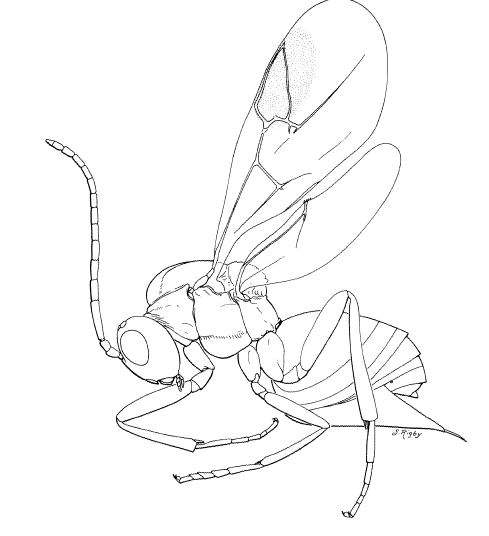
\includegraphics[width=\textwidth]{CynipidHabitus}
  \caption{Cynipidae habitus \citep[][Fig. 197]{goulet1993hymenoptera}}
  \label{fig:cynipid1}
\end{subfigure}
    \caption{Cynipoidea}\label{fig:cynipoids}
\end{figure}

\subsubsection{Cynipidae (gall wasps)}
\noindent{}\textit{Diagnostic characters:} fore wing with cell RI 3--4 times as long as wide; hind leg with tarsomere 1 not longer than remaining tarsomeres combined; petiole of metasoma hidden or wider than long (Figure \ref{fig:cynipid1}); scutellum rounded, not elaborate; \textgreater{}3 abdominal tergites visible, head always wider than mesosoma.\\

\noindent{}\textit{Natural history:} Most of the $\sim$1,300 species are gall-makers on plants or inquilines inside the galls of other insects. Many of these wasps are associated with oaks (\textit{Quercus} spp.).\\

\noindent{}The next families are classified in the super diverse taxon Chalcidoidea. We'll look at five families, but keep in mind there are more than 20 chalcidoid families worldwide, many of which are quite common in Pennsylvania. They all share the following characteristics, the combination of which separates chalcidoids from other apocritans:
\begin{itemize}
\item antenna geniculate, with ``ring segments' (\textit{i.e.}, short, ring-like sclerites at the base of the flagellum)
\item pronotum not reaching tegula (\textit{i.e.}, a sclerite (prepectus) is present between the pronotum and tegula)
\item fore wing with 3 veins, similar to Scelionidae
\end{itemize}

\subsubsection{Chalcididae (chalcidid wasps)}
\noindent{}\textit{Diagnostic characters:} Tarsi 5-segmented; hind femora greatly swollen and often toothed, hind tibiae curved to fit femora (Figure \ref{fig:chalcidid}); hind coxae much larger than front coxae (Figure \ref{fig:chalcidid}); fairly large (for chalcidoids!); very rarely (if ever) metallic in color.\\

\noindent{}\textit{Natural history:} Almost 1,500 species are known worldwide. Most are parasitoids of Lepidoptera (especially the pupa) or late instar Diptera.\\

\noindent{}\textbf{Question 5:} What do you think is/are the function(s) of the hind femora in Chalcididae? What makes them so large?\\

\begin{figure}[ht!]
  \centering
\begin{subfigure}[ht!]{0.45\textwidth}
    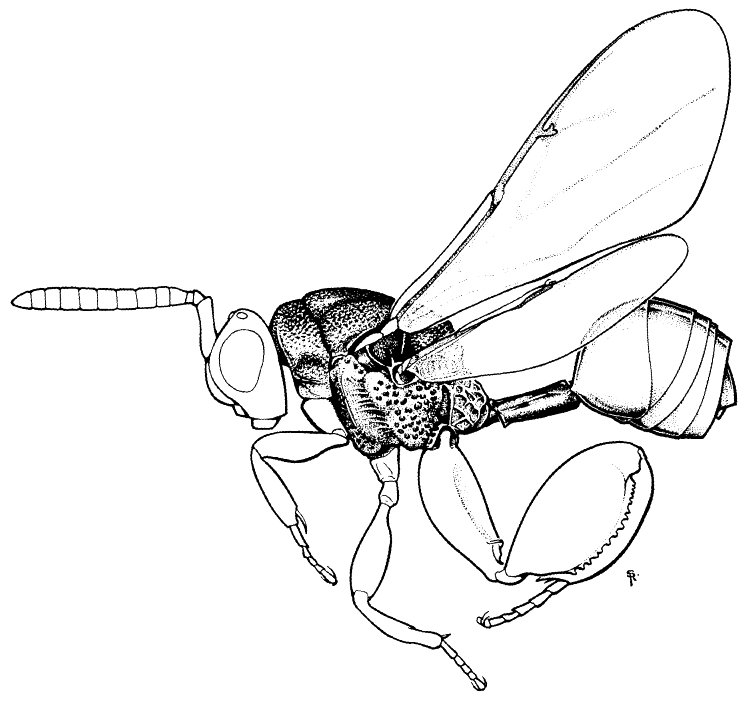
\includegraphics[width=\textwidth]{ChalcididHabitus}
  \caption{Chalcididae lateral habitus \citep[][Fig. 212]{goulet1993hymenoptera}}
  \label{fig:chalcidid}
\end{subfigure}
    \hfill
\begin{subfigure}[ht!]{0.45\textwidth}
    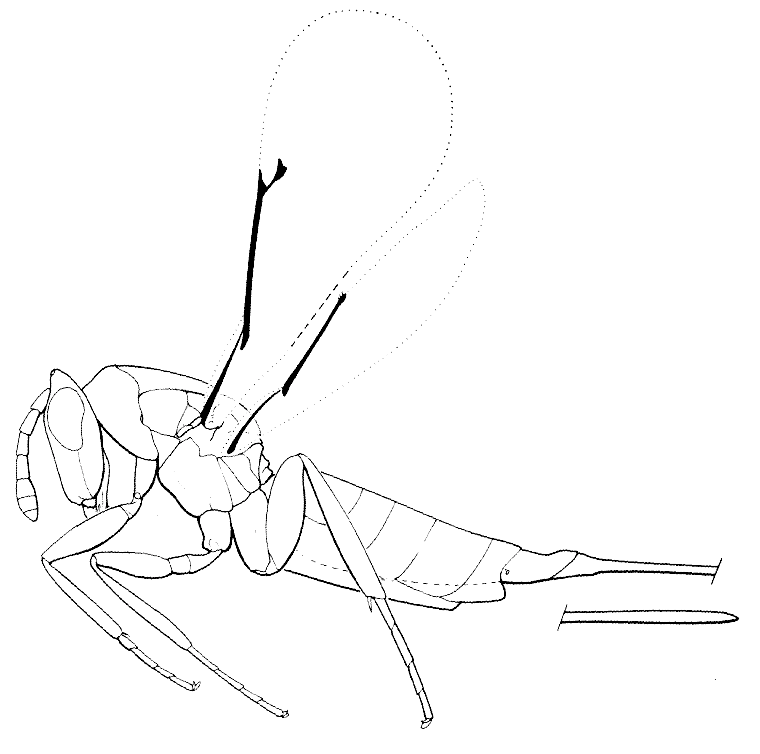
\includegraphics[width=\textwidth]{EulophidHabitus}
  \caption{Eulophidae habitus \citep[][Fig. 228]{goulet1993hymenoptera}}
  \label{fig:eulophid}
\end{subfigure}
\caption{Chalcidoidea}
\label{fig:xxxxxx}
\end{figure}

\subsubsection{Eulophidae (eulophid wasps)}
\noindent{}\textit{Diagnostic characters:} Antennal funicle with 4 or fewer antennomeres; tarsi 4-segmented (Figure \ref{fig:eulophid}); apical spur of front tibiae short and straight; small, often black, brown, or blue.\\

\noindent{}\textit{Natural history:} More than 4,300 species have been described, and they are biologically quite  diverse. Most species develop as parasitoids of other insects, especially Holometabola, but some species are gall-makers.\\

\subsubsection{Encyrtidae}
\noindent{}\textit{Diagnostic characters:} mesopleuron strongly convex, without grooves (Figure \ref{fig:encyrt1}); tarsi usually 5-segmented; if tarsi 4-segmented, funicle with 5+ antennomeres; apical spur of middle tibiae large; usually rather stout-bodied and very small; cerci distinctly anterior to apical abdominal margin (Figure \ref{fig:encyrt2}).\\

\noindent{}\textit{Natural history:} There are $\sim$3,700 described species worldwide. Like other chalcidoids, this lineage is biologically diverse. Most species are parasitoids of insect eggs or  of sternorrhynchans, and many are important biological control agents.

\begin{figure}[ht!]
  \centering
\begin{subfigure}[ht!]{0.55\textwidth}
    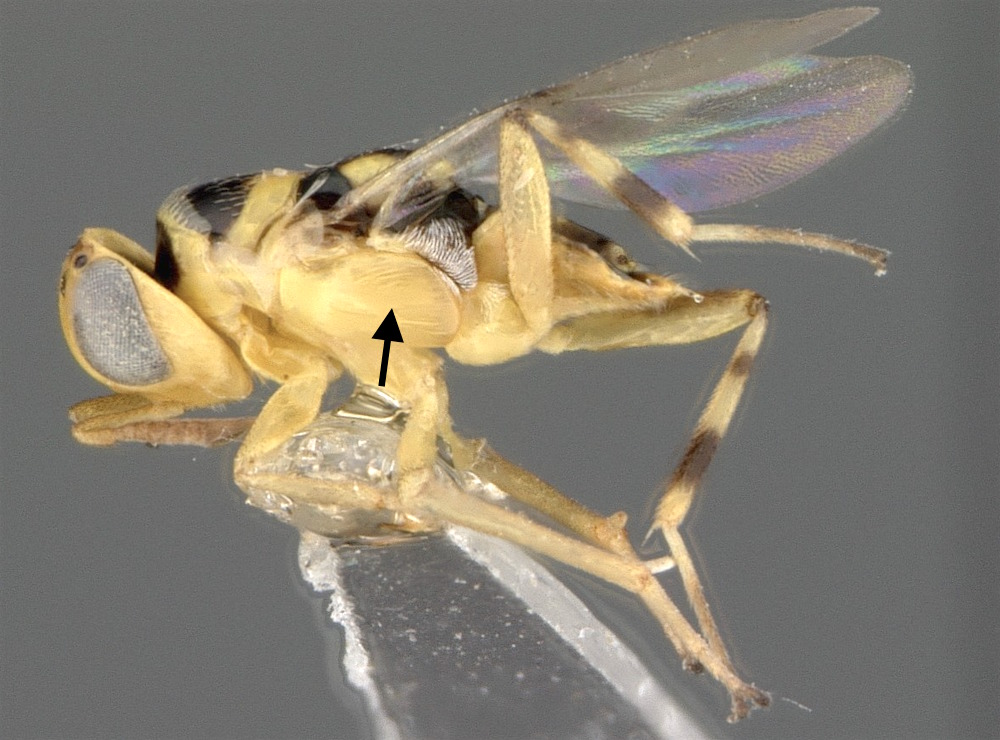
\includegraphics[width=\textwidth]{EncyrtidHabitus}
  \caption{Habitus. Photo CC0 by Michael Gates \url{http://morphbank.net/?id=228742}}
  \label{fig:encyrt1}
\end{subfigure}
    \hfill
\begin{subfigure}[ht!]{0.35\textwidth}
    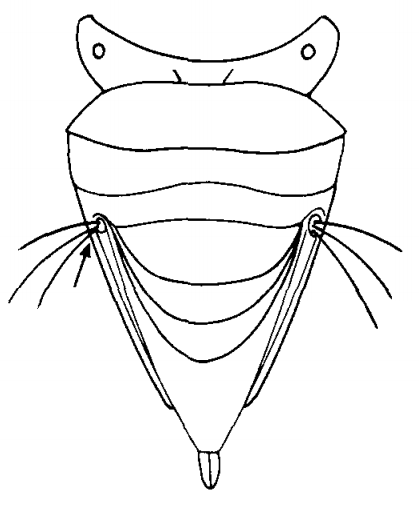
\includegraphics[width=\textwidth]{EncyrtidMetasoma}
  \caption{Metasoma in dorsal view \citep[][pg. 581]{goulet1993hymenoptera}}
  \label{fig:encyrt2}
\end{subfigure}
    \caption{Encyrtidae}\label{fig:encyrt}
\end{figure}

\subsubsection{Mymaridae (fairyflies)}
\noindent{}\textit{Diagnostic characters:} Body typically very small (these wasps are parasitoids of insect eggs); head with H-shaped complex bar-like structures on face (trabeculae); wings fringed; hind wing stalked proximally.\\

\noindent{}\textit{Natural history:} There are \textgreater1,400 known species, all of which are (probably) parasitoids of insect eggs. This family includes the smallest known insect (\textit{Dicopomorpha echmepterygis} Mockford, 1997) and the smallest known flying insect (\textit{Kikiki huna} Huber \& Noyes 2013). The facial trabeculae likely correspond to an egg-bursting structure that facilitates eclosion and escape from the host remains.

\begin{figure}[ht!]
  \centering
\begin{subfigure}[ht!]{0.5\textwidth}
    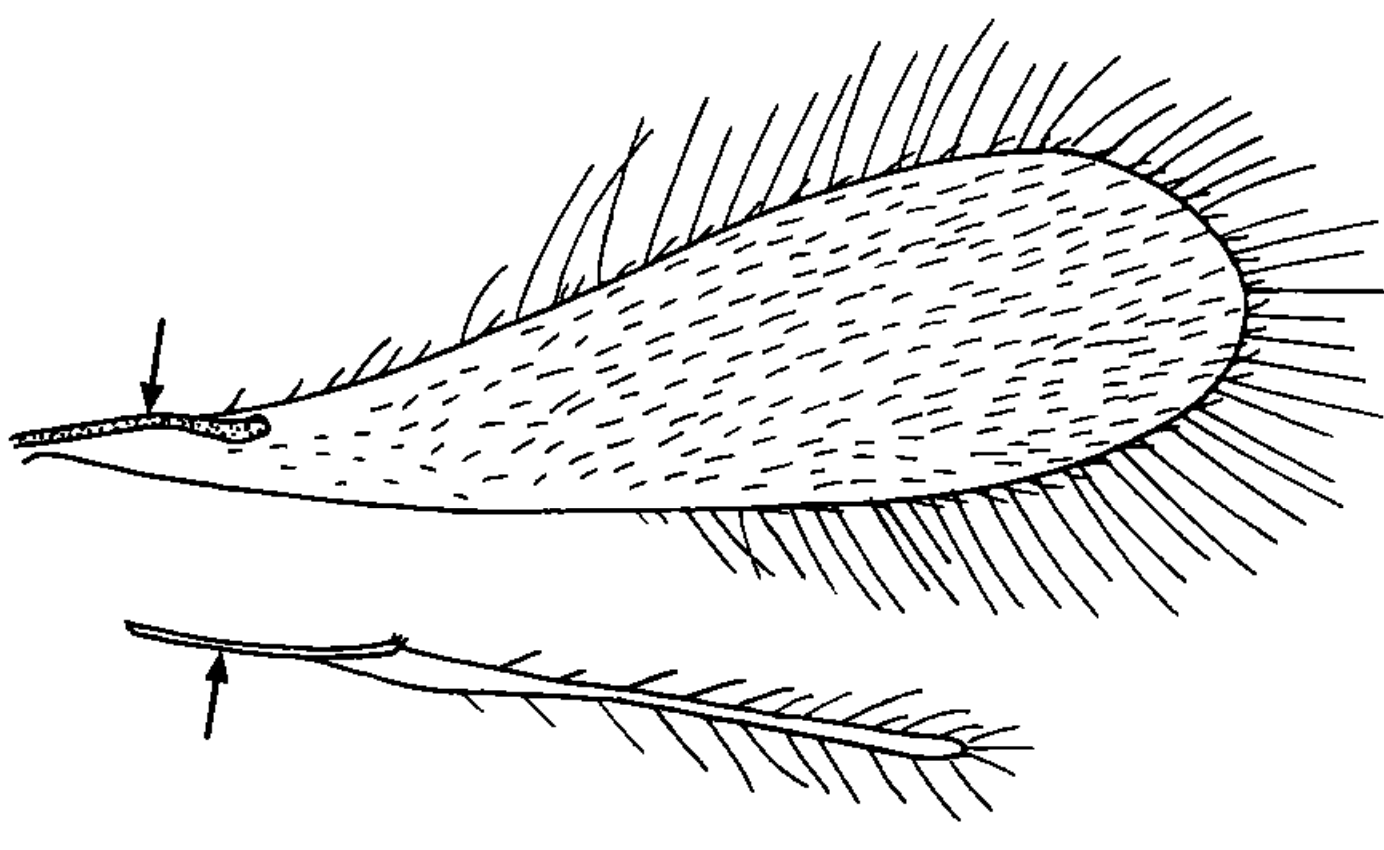
\includegraphics[width=\textwidth]{MymaridWings}
  \caption{Wings}
  \label{fig:mymarid1}
\end{subfigure}
    \qquad
\begin{subfigure}[ht!]{0.28\textwidth}
    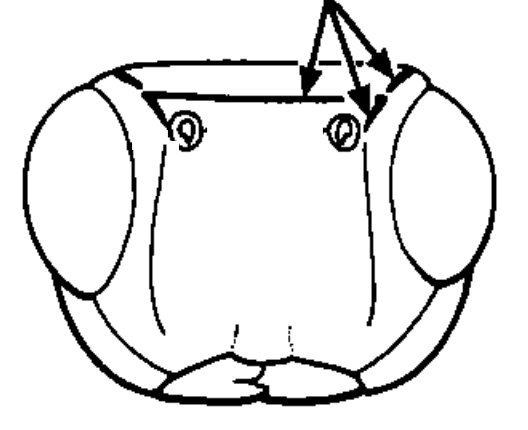
\includegraphics[width=\textwidth]{MymaridHead}
  \caption{Head in anterior view}
  \label{fig:mymarid2}
\end{subfigure}
    \caption{Mymaridae \citep[][pg. 87]{goulet1993hymenoptera}}\label{fig:mymarids}
\end{figure}

\paragraph*{Aculeata} In Aculeata, the egg does not enter the ovipositor assembly prior to deposition but rather leaves the metasoma anterior to the ovipositor. The ovipositor functions only to inject venom gland products (\textit{i.e.}, venom). Besides the structure of the ovipositor, the monophyly of Aculeata is supported mostly by indistinct internal characters (\textit{e.g.}, the shape, pattern and presence/absence of thoracic muscles). The only distinct synapomorphy of the infraorder is the presence of the supramesopleural sclerite (sms), that partially obscures the second thoracic spiracle. (Caveat: The sms is absent from a few Aculeata and \textit{present} in some non-aculeates, like Evaniidae and Trigonalidae.)

Besides the above-mentioned synapomorphies, Aculeata can be superficially characterized by their well-developed wing venation (but see some ``Chrysidoidea''), distinct wasp waist (unlike sawflies), well sclerotized metasomal sternites (unlike most Ichneumonoidea), having fewer than 11 flagellomeres (numerous Ichneumonoidea have more than 11 flagellomeres), and convex, almost bulbous metasoma.

Traditionally the infraorder is subdivided into three superfamilies: Chrysidoidea, Apoidea, and Vespoidea. Only the monophyly of Apoidea is supported in the latest phylogenetic analyses.

\subsubsection{Bethylidae}
\noindent{}\textit{Diagnostic characters:} Body usually weakly sculptured and brown or black (not typically metallic); head usually prognathous (Figure \ref{fig:bethylid1}); antenna with 11 (rarely 10 or 8) flagellomeres; pronotum with anterior flange, propleuron thus concealed in dorsal view; distal venation of wing reduced; metasoma with 6 or 7 exposed terga. \\

\noindent{}\textit{Natural history:} \\

\begin{figure}[ht!]
  \centering
\begin{subfigure}[ht!]{0.28\textwidth}
    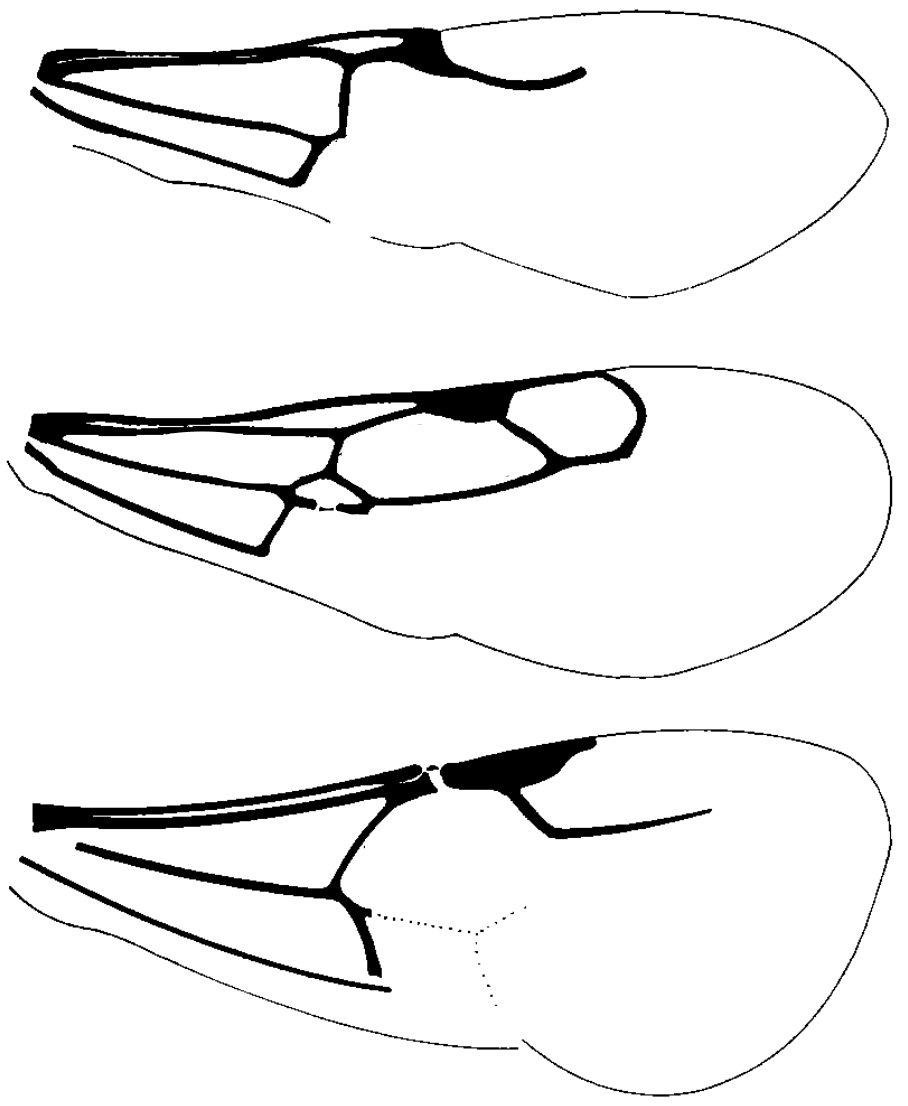
\includegraphics[width=\textwidth]{BethylidWings}
  \caption{Fore wings \citep[][pg. 134]{goulet1993hymenoptera}}
  \label{fig:bethylid1}
\end{subfigure}
    \qquad
\begin{subfigure}[ht!]{0.35\textwidth}
    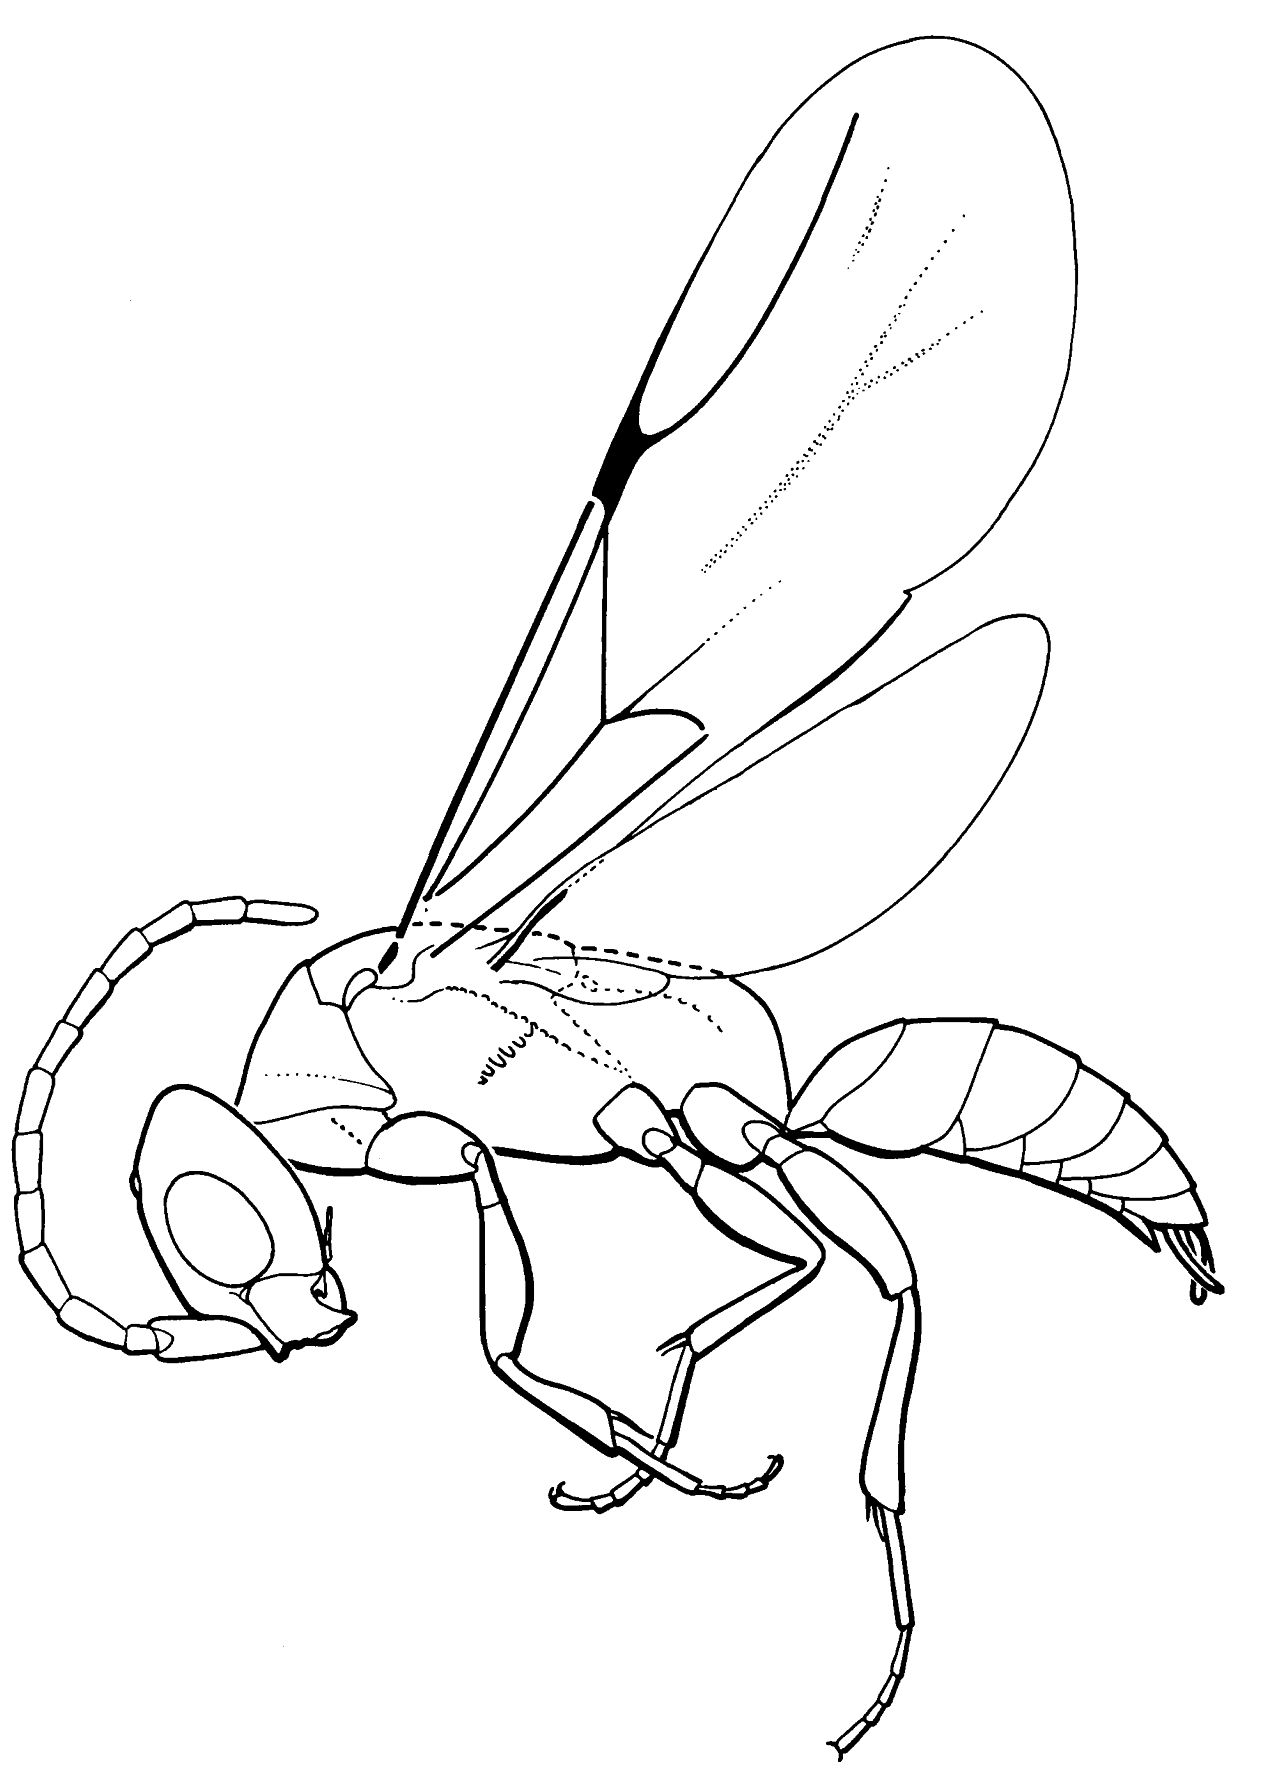
\includegraphics[width=\textwidth]{BethylidHabitus}
  \caption{Habitus \citep[][Fig. 37]{goulet1993hymenoptera}}
  \label{fig:bethylid2}
\end{subfigure}
    \caption{Bethylidae}\label{fig:bethylids}
\end{figure}

\subsubsection{Chrysididae (cuckoo wasps)}
\noindent{}\textit{Diagnostic characters:} Head typically hypognathous; antenna with 11 flagellomeres; pronotum with anterior flange, thus propleuron concealed in dorsal view; pronotum with posterolateral apex usually well separated from tegula but sometimes touching; metasoma usually with 5 or fewer exposed terga; strongly concave ventrally (Figure \ref{fig:chrysididae}); usually strongly sculptured; usually metallic (Figure \ref{fig:chrysid1})\\

\noindent{}\textit{Natural history:} \\

\begin{figure}[ht!]
    \centering
    \begin{subfigure}[ht!]{0.42\textwidth}
        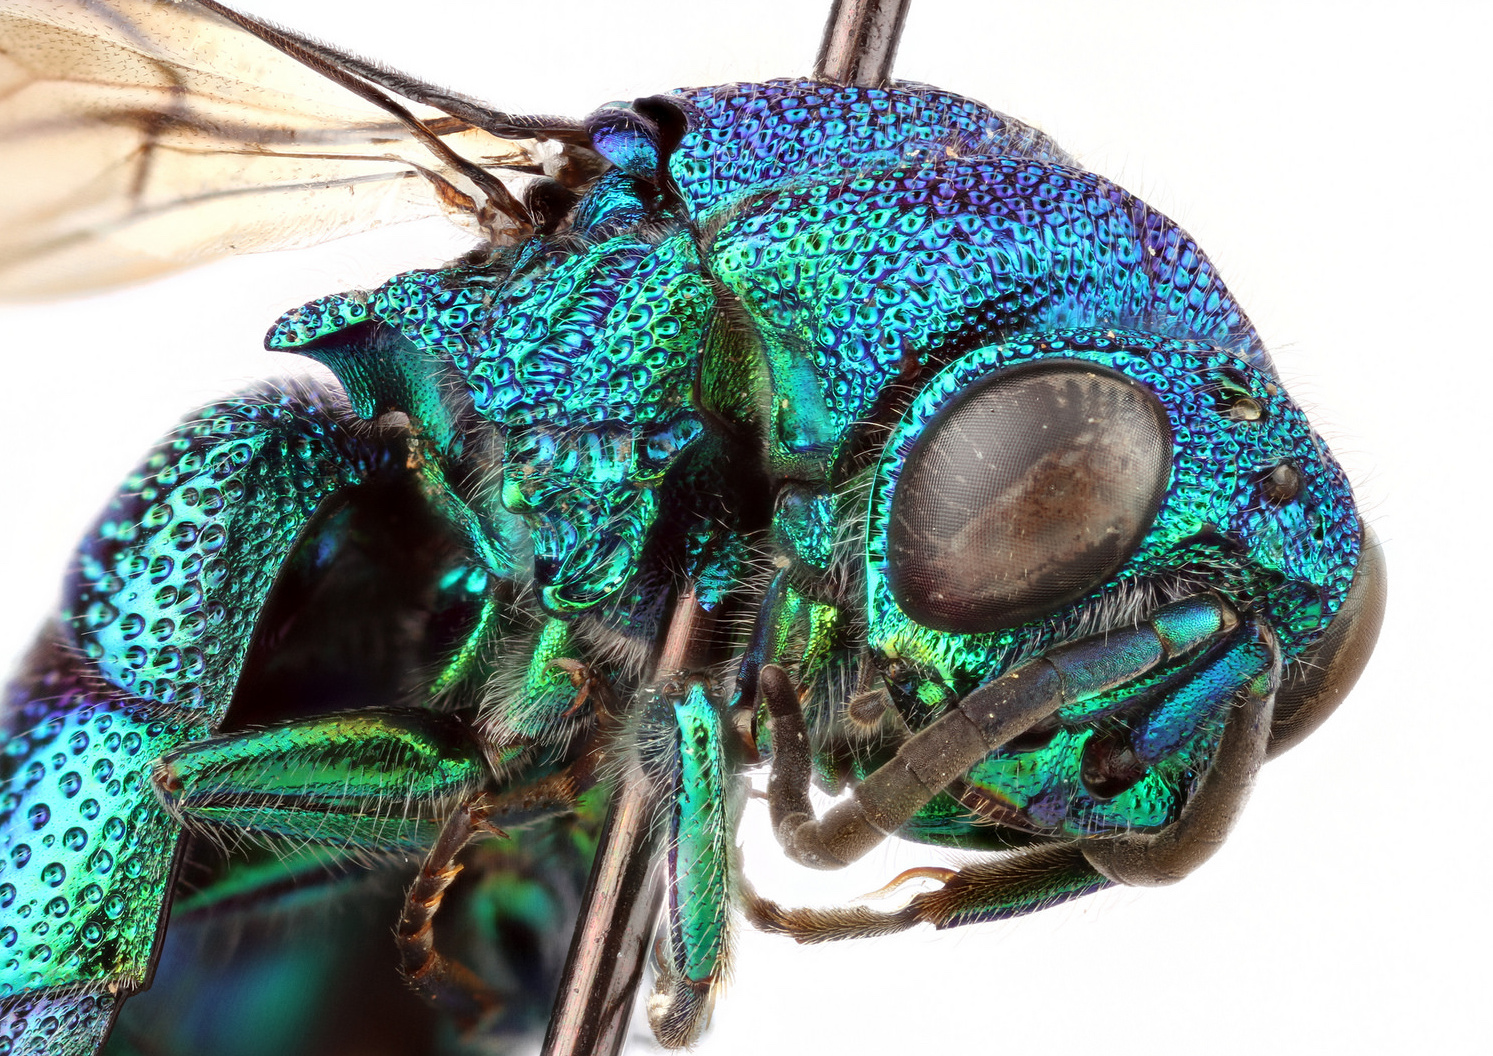
\includegraphics[width=\textwidth]{ChrysididColor}
        \caption{Habitus. Photo CC0 by James Marchment \url{https://flic.kr/p/DciZEn}}
        \label{fig:chrysid1}
    \end{subfigure}
    \qquad
    \begin{subfigure}[ht!]{0.39\textwidth}
        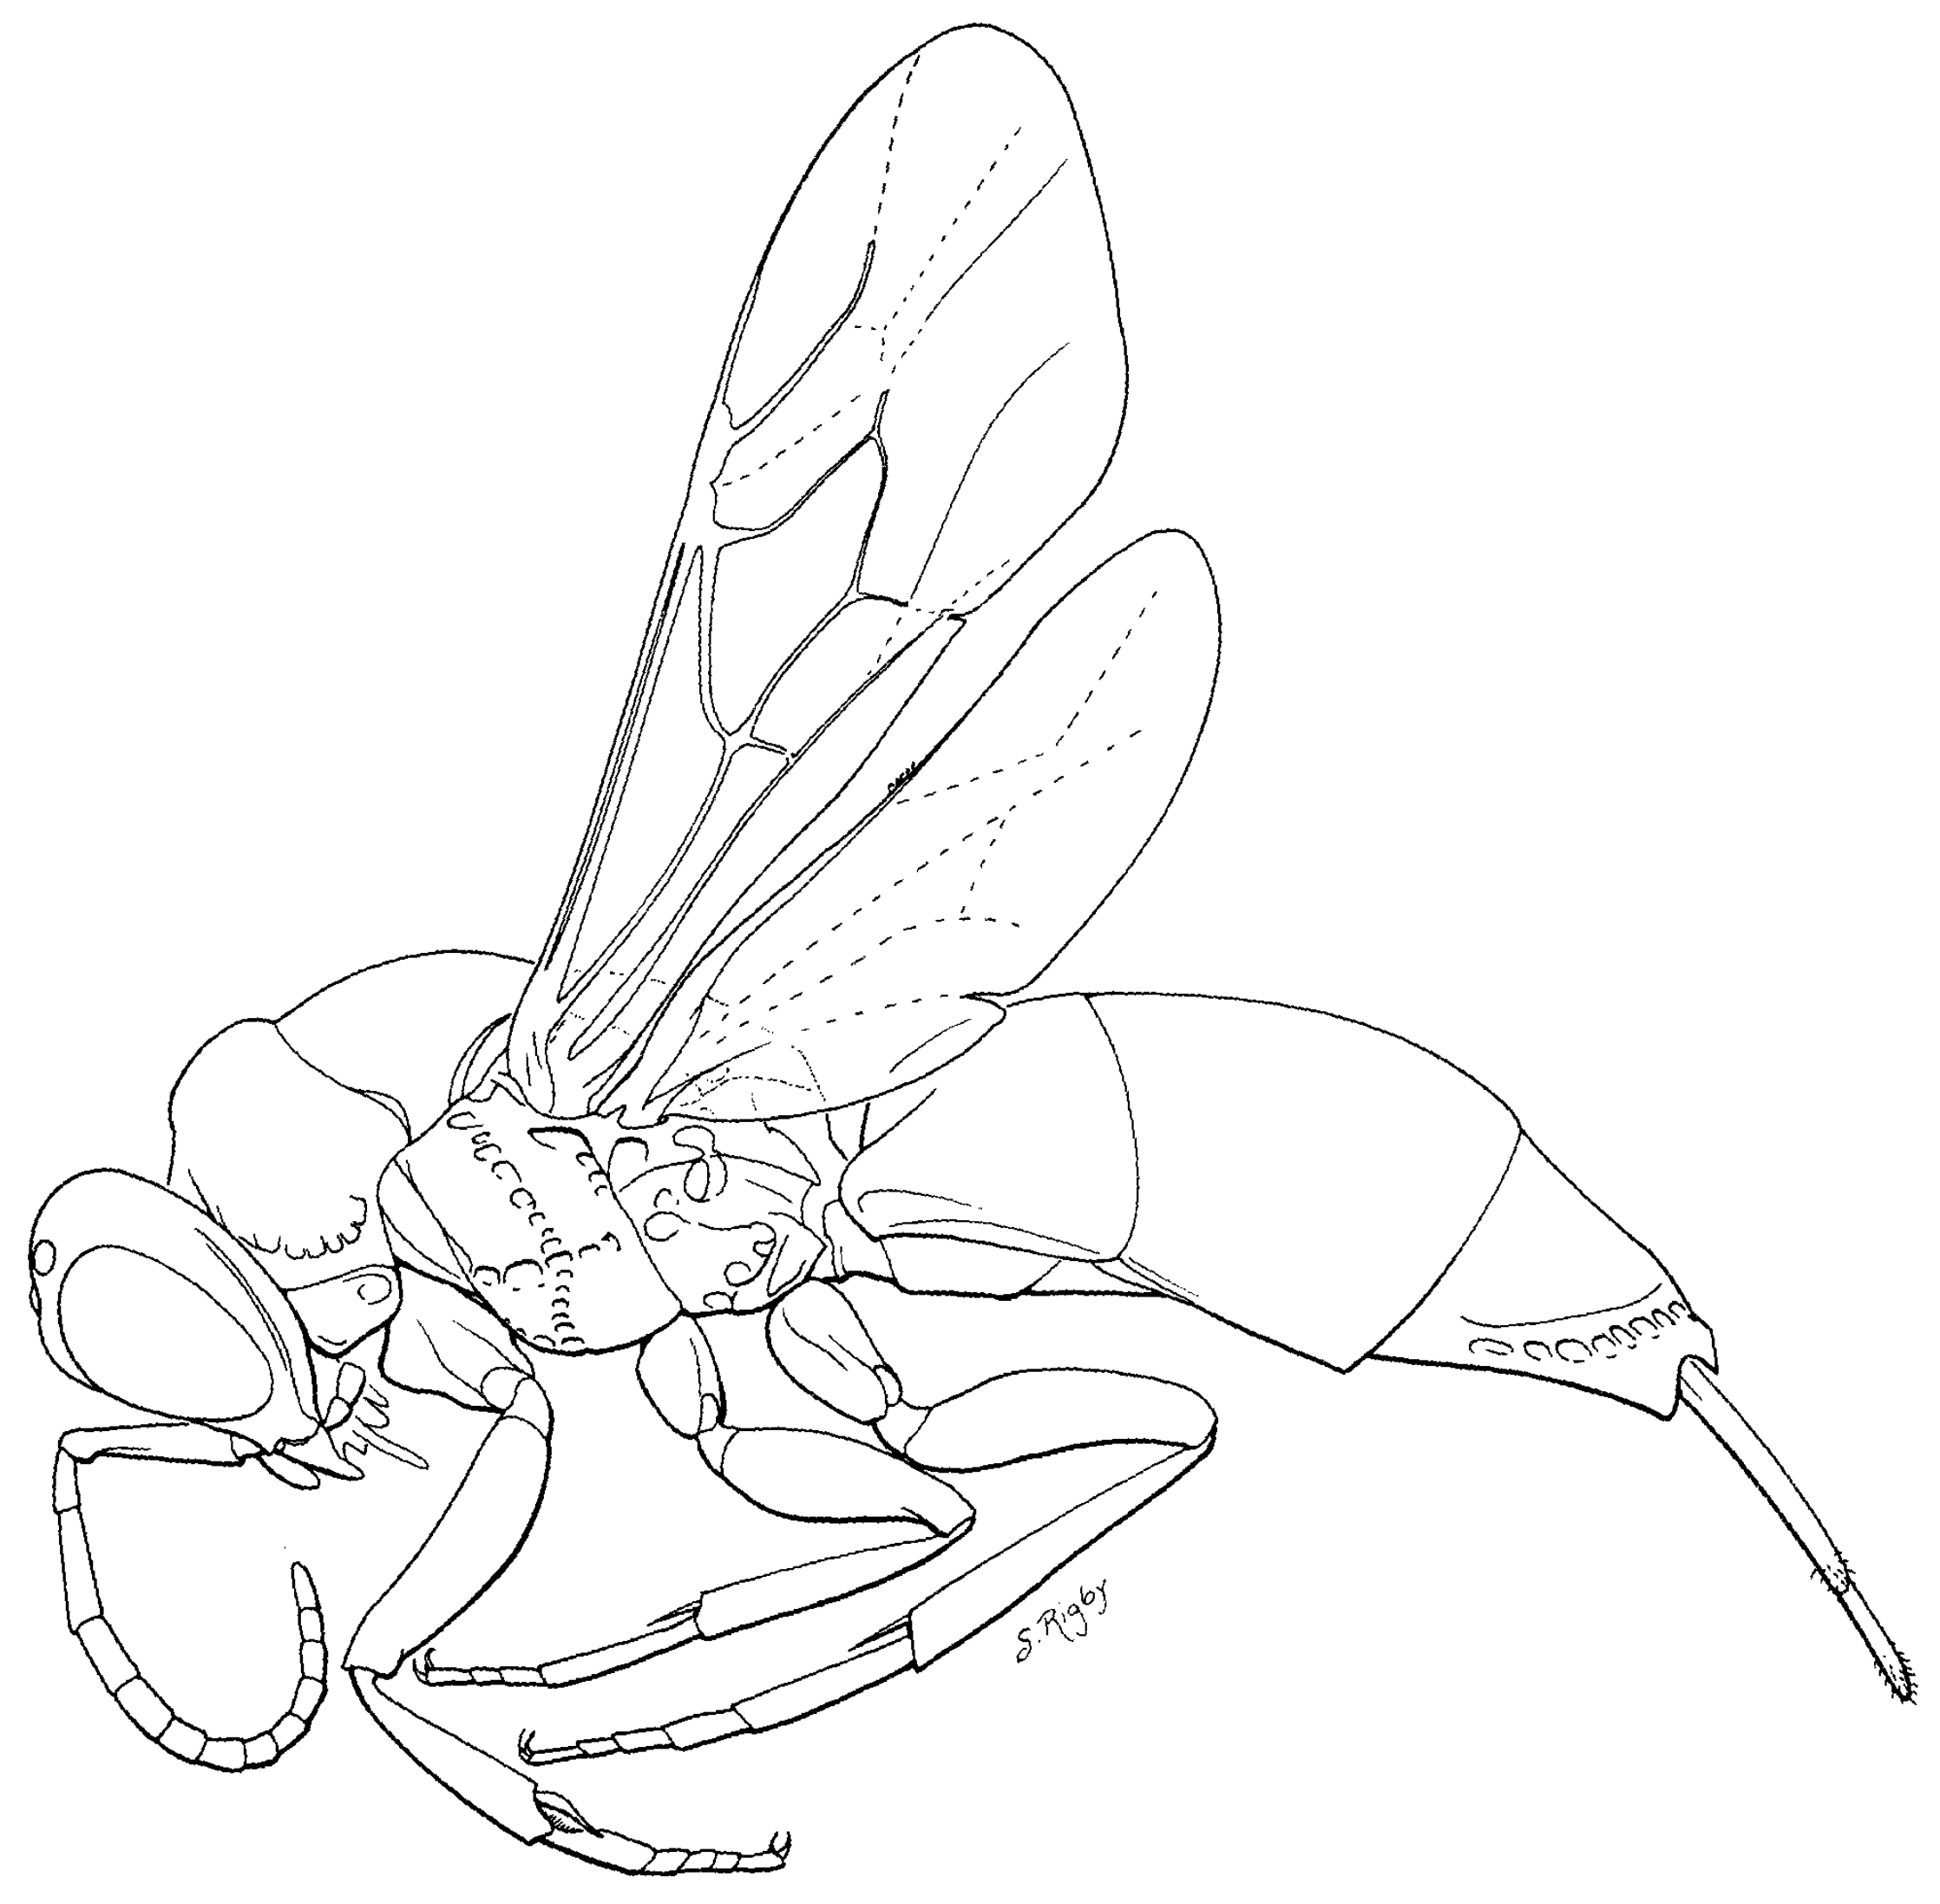
\includegraphics[width=\textwidth]{ChrysididHabitus}
        \caption{Habitus \citep[][Fig. 42]{goulet1993hymenoptera}}
        \label{fig:chrysid2}
    \end{subfigure}
    \caption{Chrysididae}\label{fig:chrysididae}
\end{figure}
\FloatBarrier

\noindent{}The next six families are usually classified in Vespoidea, a taxon comprising 2--11 extant families, depending on whom you ask. Many species are parasitoids, but we're starting to see some that are predators (Vespidae), even pollen gatherers (Vespidae: Masarinae), or with broadly diverse diets (Formicidae). And many species are highly eusocial (many Vespidae, all Formicidae). 

\subsubsection{Tiphiidae}
\noindent{}\textit{Diagnostic characters:} eye not usually ``notched'', like we see in Vespidae; mesosternum with laminate expansions on each side of midline covering bases of contiguous mesocoxae, the expansions rarely reduced to small teeth; hind wing with deeply separated (jugal) lobe (Figure \ref{fig:tiphiid2}); female usually with mesotibia and metatibia stout and spiny; metasomal segment 1 without a true node (like we see in Formicidae), although sometimes approaching it; male metasomal sternum 8 (hypopygium) usually forming a single strong acute, upcurved hook, the hypopygium sometimes simple or with 2--5 spines, and usually entirely exposed (Figure \ref{fig:tiphiidae}).\\

\noindent{}\textit{Natural history:} \\

\begin{figure}[ht!]
    \centering
    \begin{subfigure}[ht!]{0.4\textwidth}
        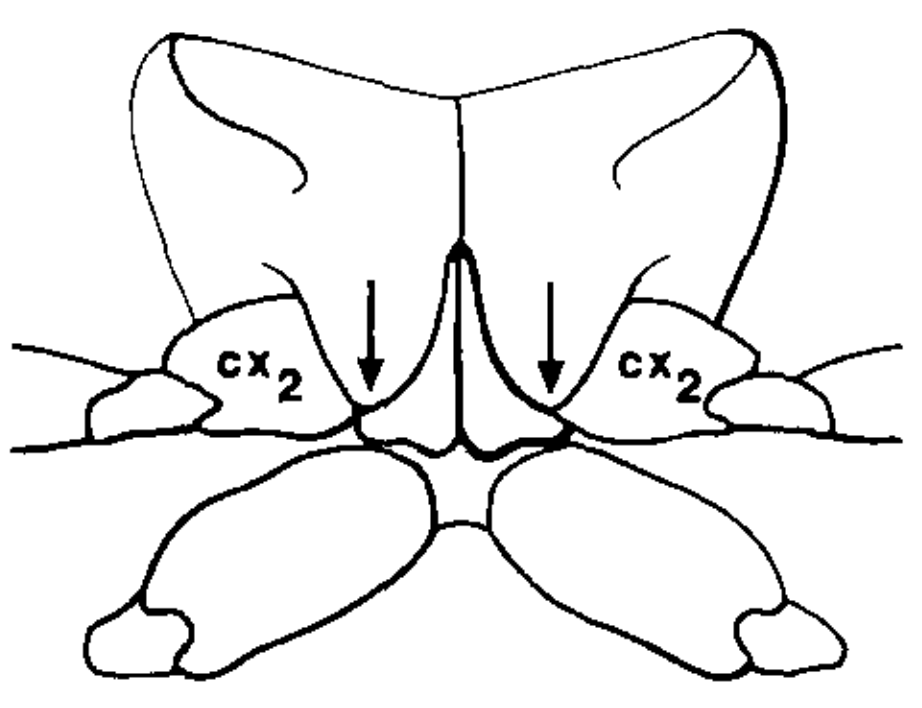
\includegraphics[width=\textwidth]{TiphiidMesosoma}
        \caption{Mesosoma in venral view \citep[][pg. 163]{goulet1993hymenoptera}; cx2 = mesocoxa}
        \label{fig:tiphiid1}
    \end{subfigure}
    \qquad
    \begin{subfigure}[ht!]{0.45\textwidth}
        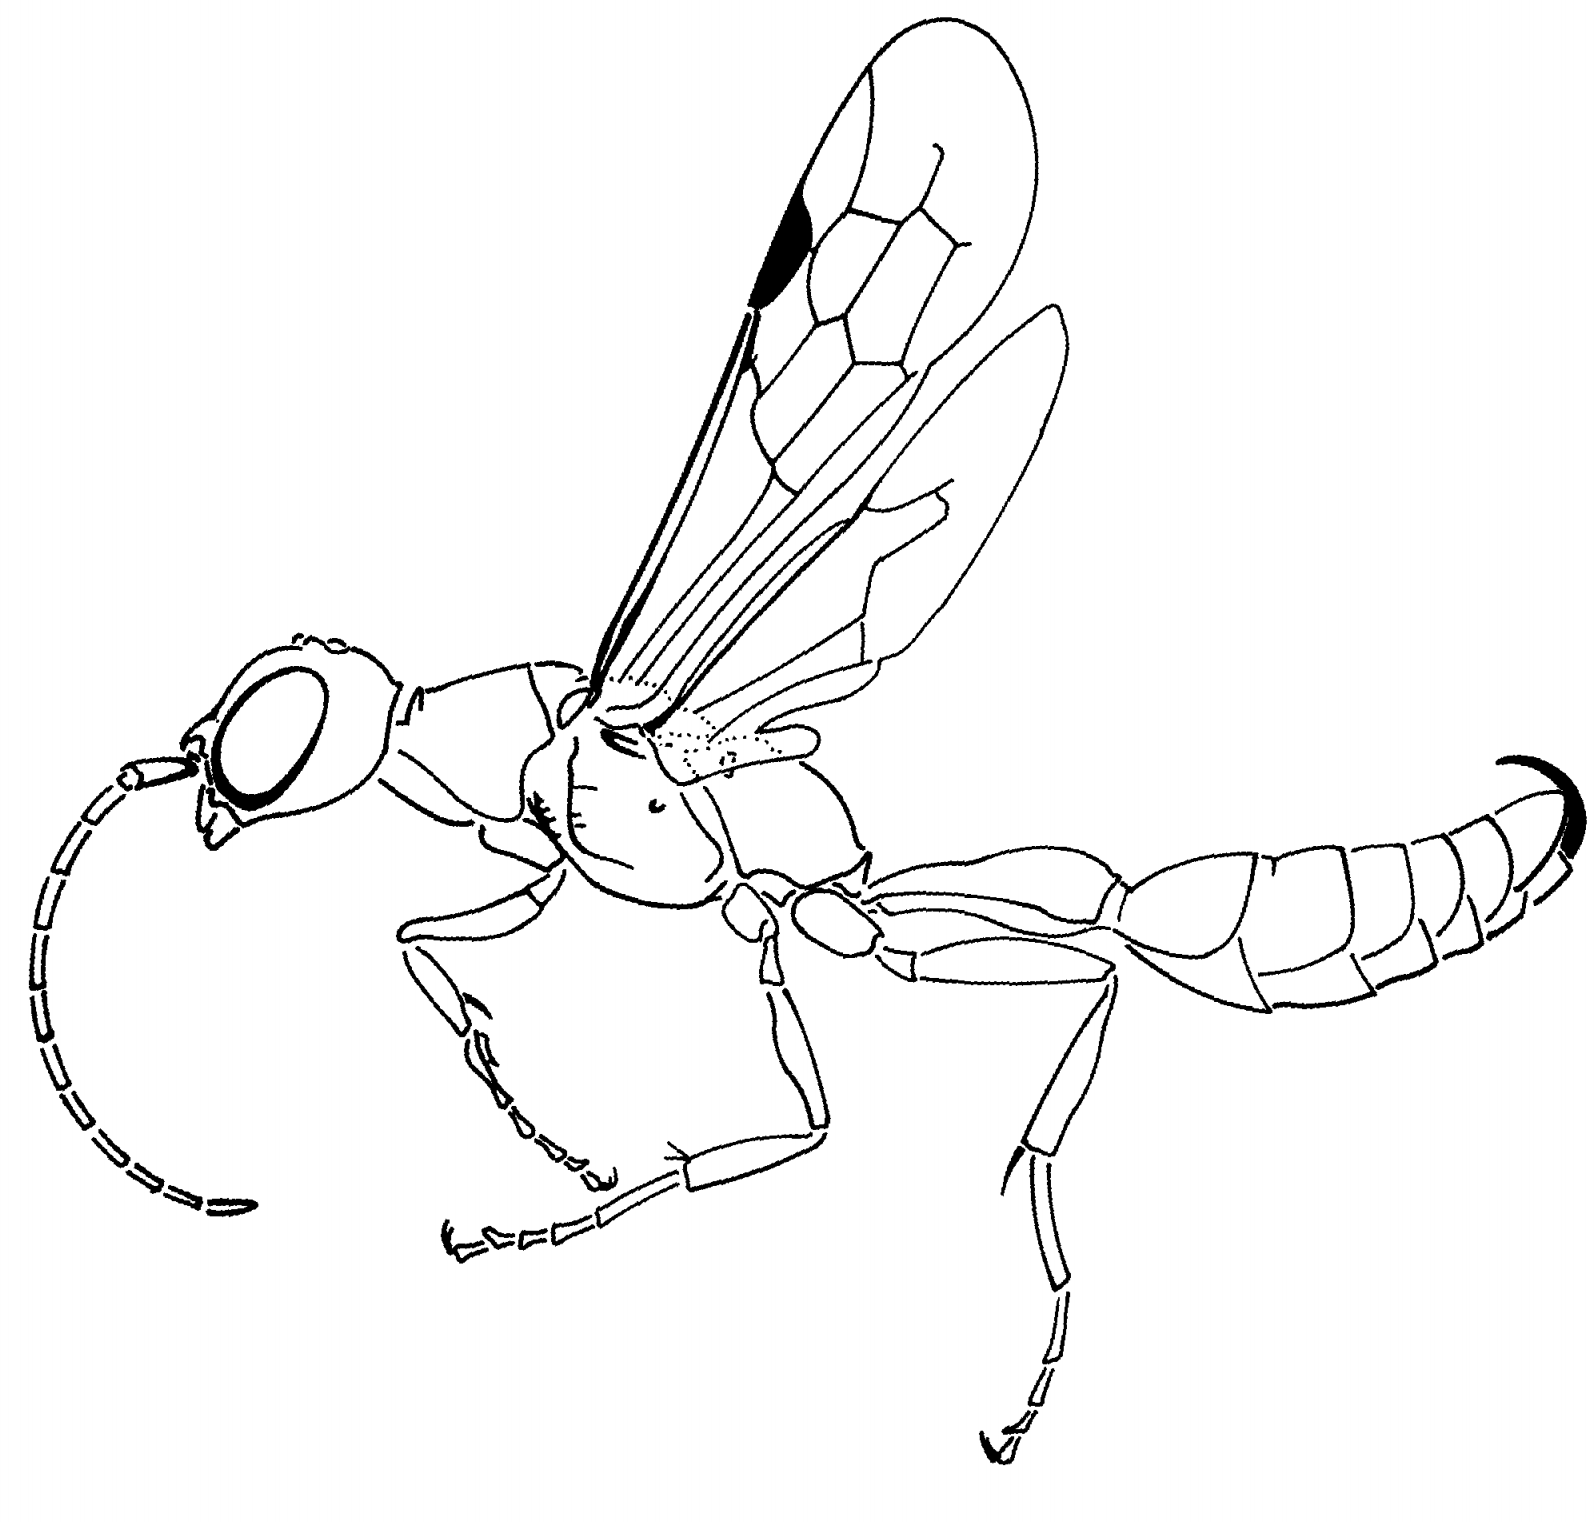
\includegraphics[width=\textwidth]{TiphiidHabitus}
        \caption{Habitus \citep[][Fig. 49]{goulet1993hymenoptera}}
        \label{fig:tiphiid2}
    \end{subfigure}
    \caption{Tiphiidae}\label{fig:tiphiidae}
\end{figure}

\subsubsection{Mutillidae (velvet ants)}
\noindent{}\textit{Diagnostic characters:} metasomal segment 1 without a true node; metasomal segment 2 usually with longitudinal felt line or with felted pit on tergum and/or sternum (but sometimes without); female almost always apterous (Figure \ref{fig:mutillid1}); apterous forms with pronotum usually fused to mesothorax and mesonotum to metanotum-propodeum complex; usually very furry and often colorful or brownish and quite ``bristly''; body often very hard and difficult to pin.\\

\noindent{}\textit{Natural history:} Why are velvet ants typically brightly colored? Keep in mind that their stings are quite long (and painful!). Based on their lack of wings (in females, at least) and the \textit{very} heavily sclerotized bodies what would you hypothesize about their life histories?\\

\begin{figure}[ht!]
    \centering
    \begin{subfigure}[ht!]{0.45\textwidth}
        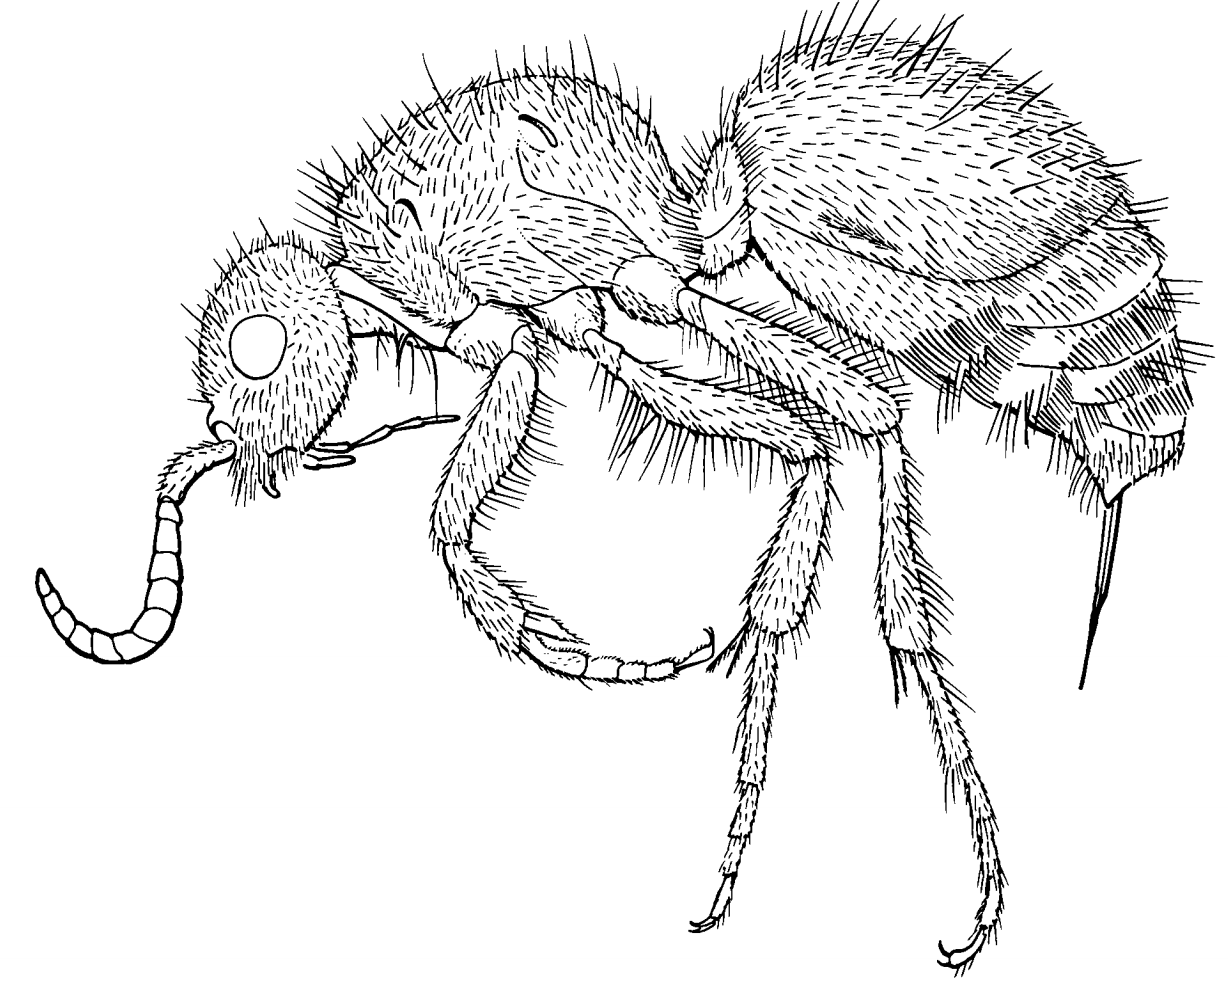
\includegraphics[width=\textwidth]{MutillidHabitus}
        \caption{Female habitus \citep[][Fig. 63]{goulet1993hymenoptera}}
        \label{fig:mutillid1}
    \end{subfigure}
    \qquad
    \begin{subfigure}[ht!]{0.45\textwidth}
        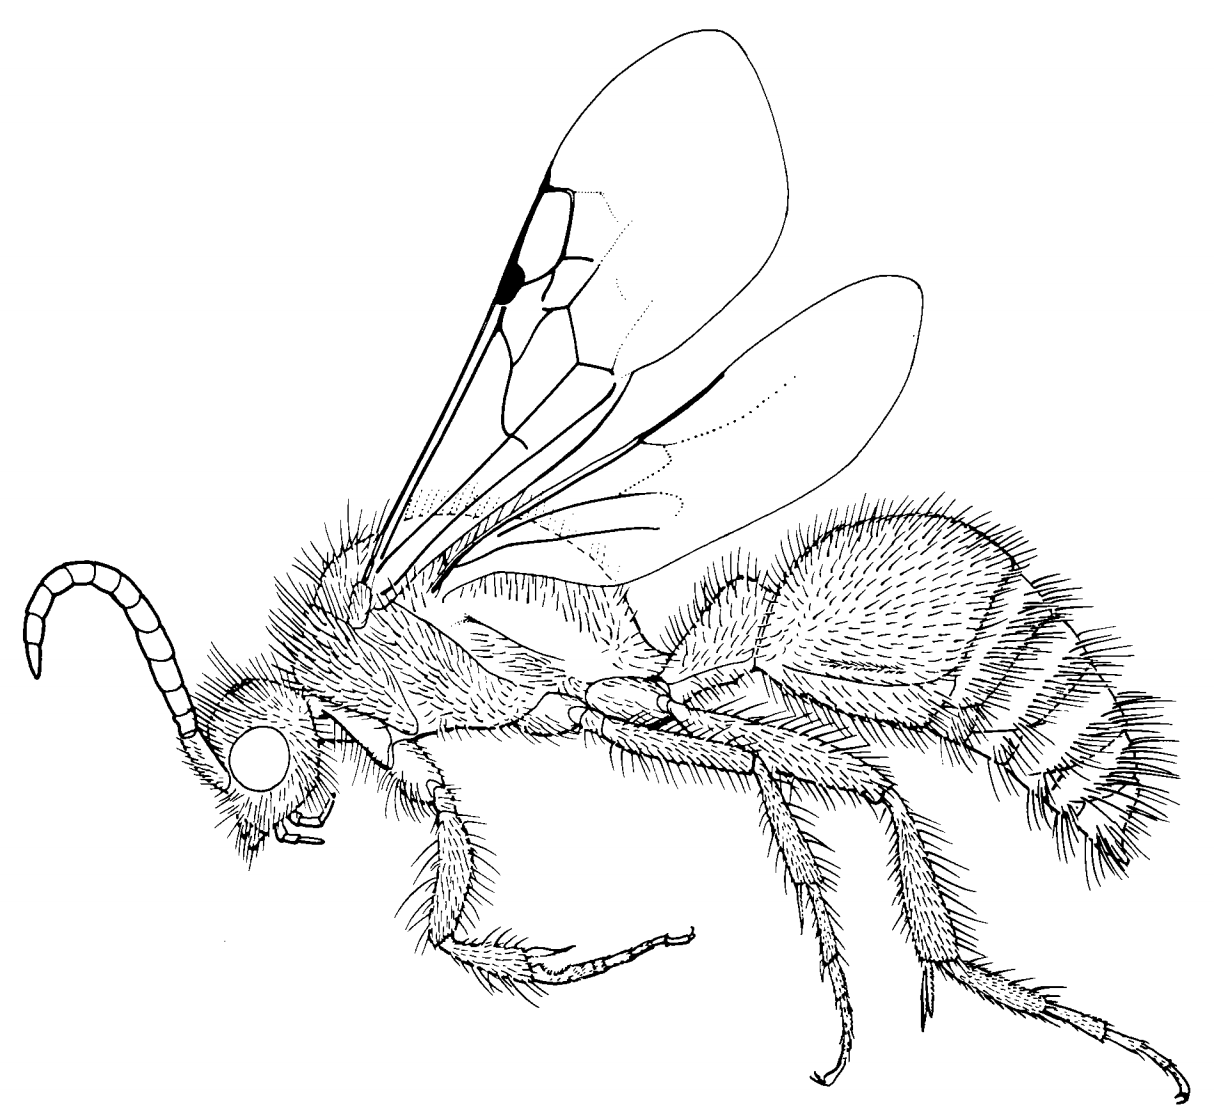
\includegraphics[width=\textwidth]{MaleMutillidHabitus}
        \caption{Male habitus \citep[][Fig. 64]{goulet1993hymenoptera}}
        \label{fig:mutillid2}
    \end{subfigure}
    \caption{Mutillidae}\label{fig:mutillids}
\end{figure}

\subsubsection{Formicidae (ants)}
\noindent{}\textit{Diagnostic characters:} Metapleural gland present (in most species), its opening usually distinct; posterior (inner) spur of metatibia modified as a calcar; reproductive forms usually macropterous, sterile female apterous; apterous form with with pronotum usually freely articulating but sometimes fused with mesothorax; mesonotum and metathorax-propodeum complex usually fused (Figure \ref{fig:formicid1}; metasoma petiolate; metasomal segment 1 usually strongly constricted at each end, forming a true node; metasomal sternum 1 separated from sternum 2 by a deep constriction.\\

\noindent{}\textit{Natural history:} Compare apterous specimens to those with wings (alates, or reproductives). Do you see differences in their mesosomal morphology? \\

\noindent{}Do you see any morphological evidence that these insects, ants, are highly eusocial? Remember the three main conditions of eusociality ...\\

\begin{figure}[ht!]
    \centering
    \begin{subfigure}[ht!]{0.42\textwidth}
        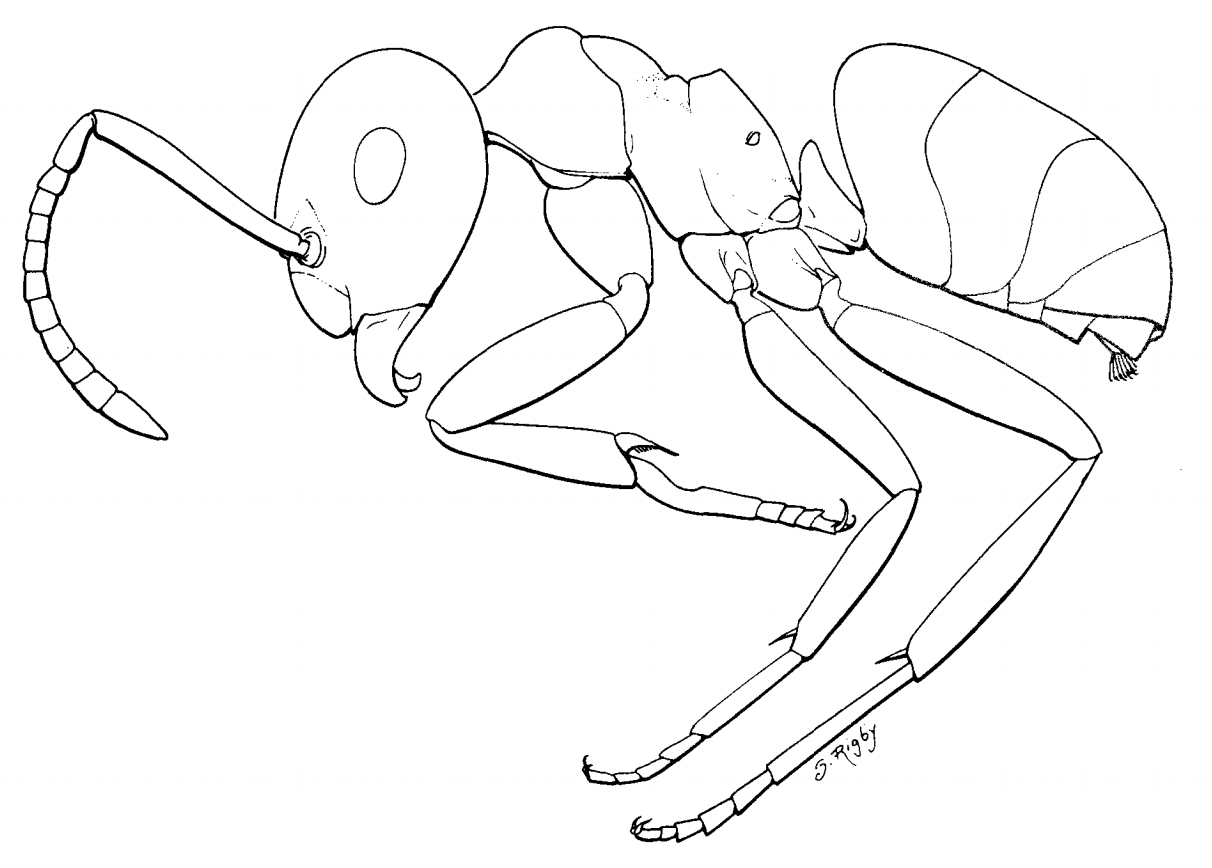
\includegraphics[width=\textwidth]{FemaleFormicidHabitus}
        \caption{Female habitus \citep[][Fig. 91]{goulet1993hymenoptera}}
        \label{fig:formicid1}
    \end{subfigure}
    \qquad
    \begin{subfigure}[ht!]{0.35\textwidth}
        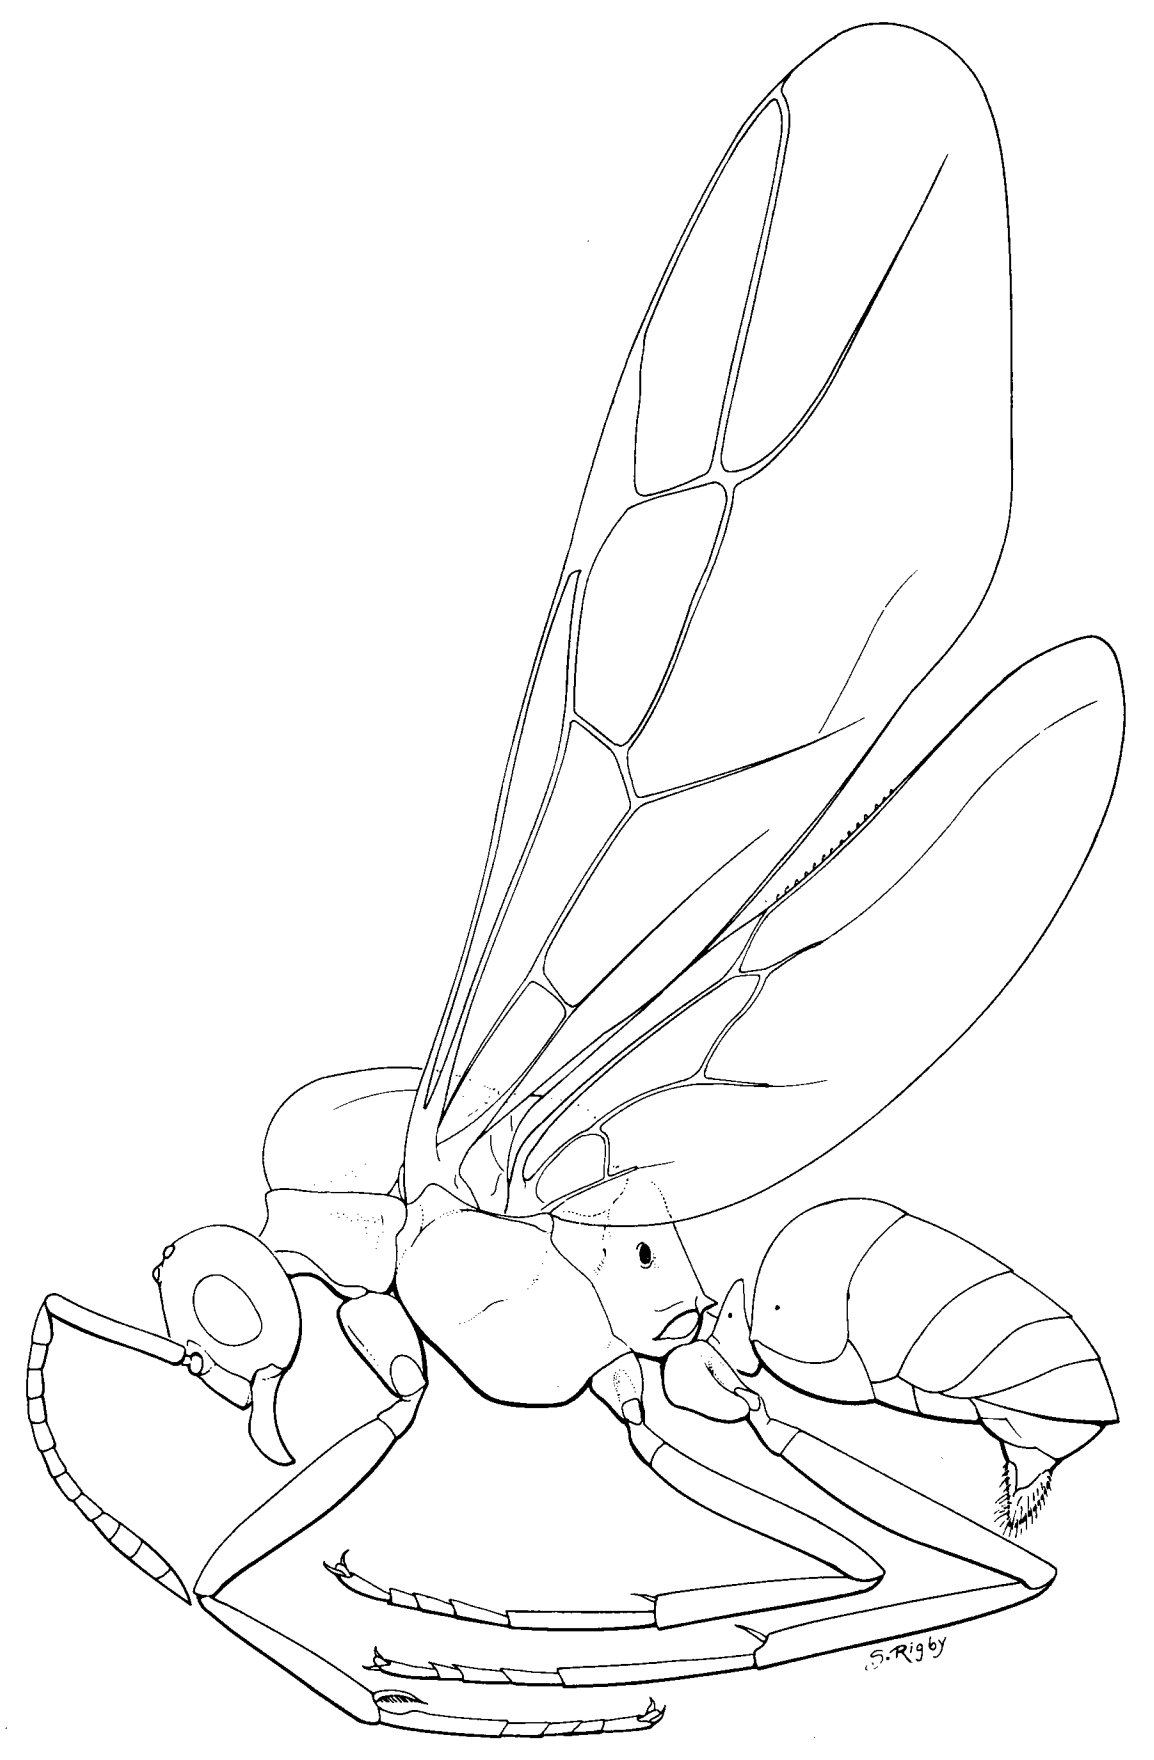
\includegraphics[width=\textwidth]{MaleFormicidHabitus}
        \caption{Male habitus \citep[][Fig. 92]{goulet1993hymenoptera}}
        \label{fig:formicid2}
    \end{subfigure}
    \caption{Formicidae}\label{fig:formicids}
\end{figure}

\subsubsection{Pompilidae (spider wasps)}
\noindent{}\textit{Diagnostic characters:} Antennal segments distinctly separated and often curled in dead specimens; pronotum with posterolateral apex rounded anterior to tegula; mesopleuron usually with oblique sulcus (Figure \ref{fig:pompilid2}); mesosoma usually laterally flattened (\textit{i.e.}, mesosoma higher than wide in anterior or posterior view); hind wing without distinct claval lobe but with distinct jugal lobe (Figure \ref{fig:pompilid3}); legs usually conspicuously elongate, spiny.\\

\noindent{}\textit{Natural history:} \\

\begin{figure}[ht!]
    \centering
    \begin{subfigure}[ht!]{0.32\textwidth}
        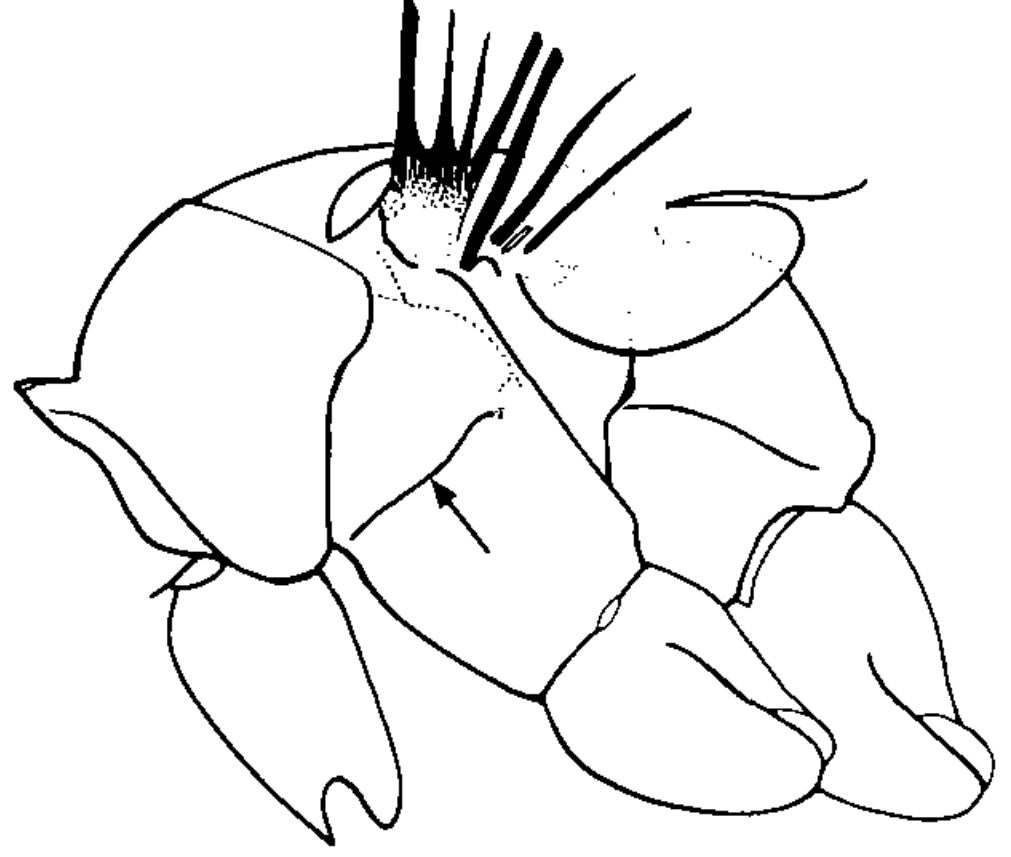
\includegraphics[width=\textwidth]{PompilidMesosoma}
        \caption{Mesosoma, with mesopleural sulcus (arrow) \citep[][pg. 170]{goulet1993hymenoptera}}
        \label{fig:pompilid2}
    \end{subfigure}
    \qquad
    \begin{subfigure}[ht!]{0.38\textwidth}
        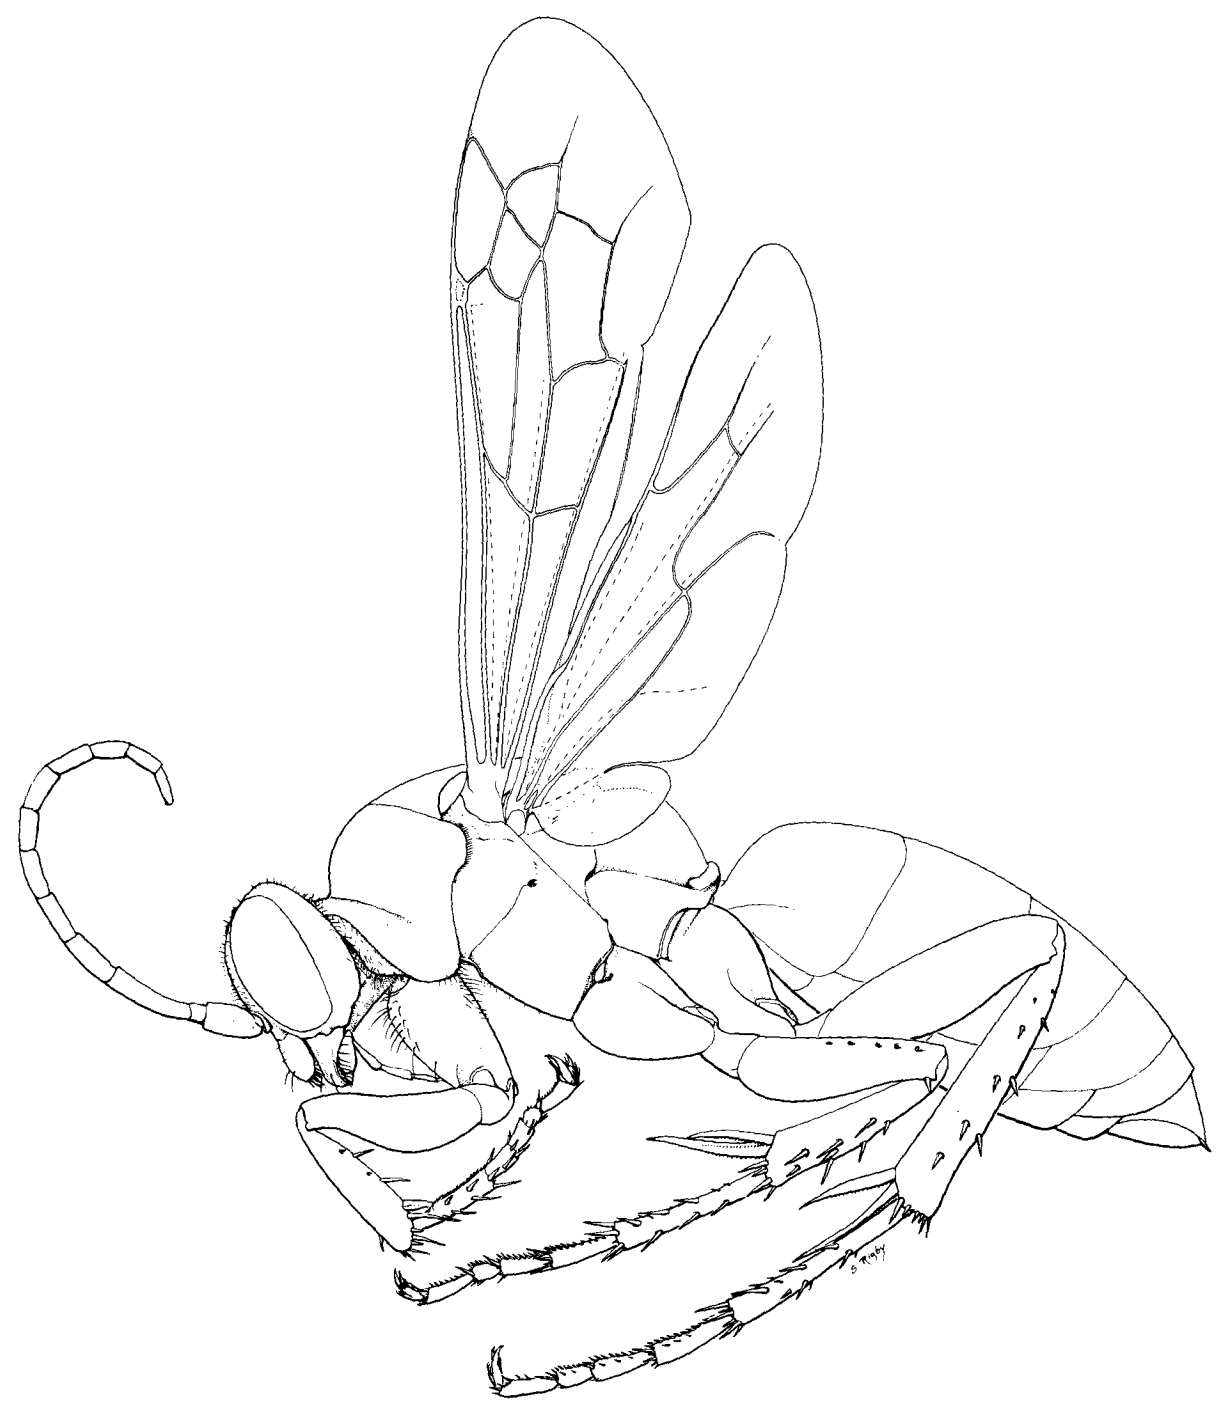
\includegraphics[width=\textwidth]{PompilidHabitus}
        \caption{Habitus \citep[][Fig. 71]{goulet1993hymenoptera}}
        \label{fig:pompilid3}
    \end{subfigure}
    \caption{Pompilidae}\label{fig:pompilid}
\end{figure}

\subsubsection{Scoliidae}
\noindent{}\textit{Diagnostic characters:} Eye with inner margin deeply emarginated (``notched''); pronotum with posterodorsal margin U-shaped; pronotum posterolateral apex truncate and weakly produced above anterior margin of tegula; mesocoxae and metacoxa widely separated; wings with dense fine longitudinal wrinkles near apices (Figure \ref{fig:scoliid1}); hind wing without distinct claval lobe but with distinct jugal lobe
female usually with mesotibia and metatibia stout and spiny; metasomal sternum 1 separated from sternum 2 by a deep constriction.\\

\noindent{}\textit{Natural history:} \\

\begin{figure}[ht!]
    \centering
    \begin{subfigure}[ht!]{0.28\textwidth}
        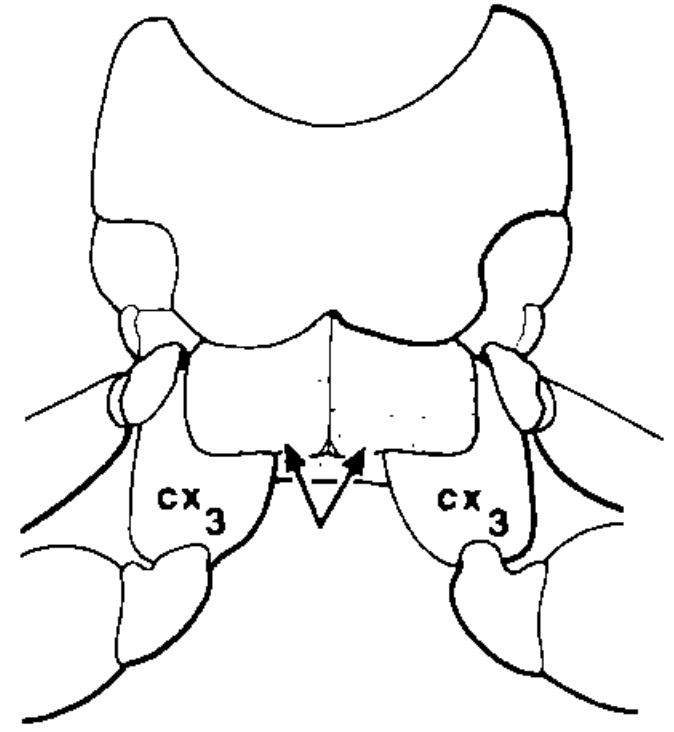
\includegraphics[width=\textwidth]{ScoliidMesosoma}
        \caption{Mesosoma in ventral view \citep[][pg. 162]{goulet1993hymenoptera}; cx3 = metacoxa}
        \label{fig:scoliid1}
    \end{subfigure}
    \qquad
    \begin{subfigure}[ht!]{0.38\textwidth}
        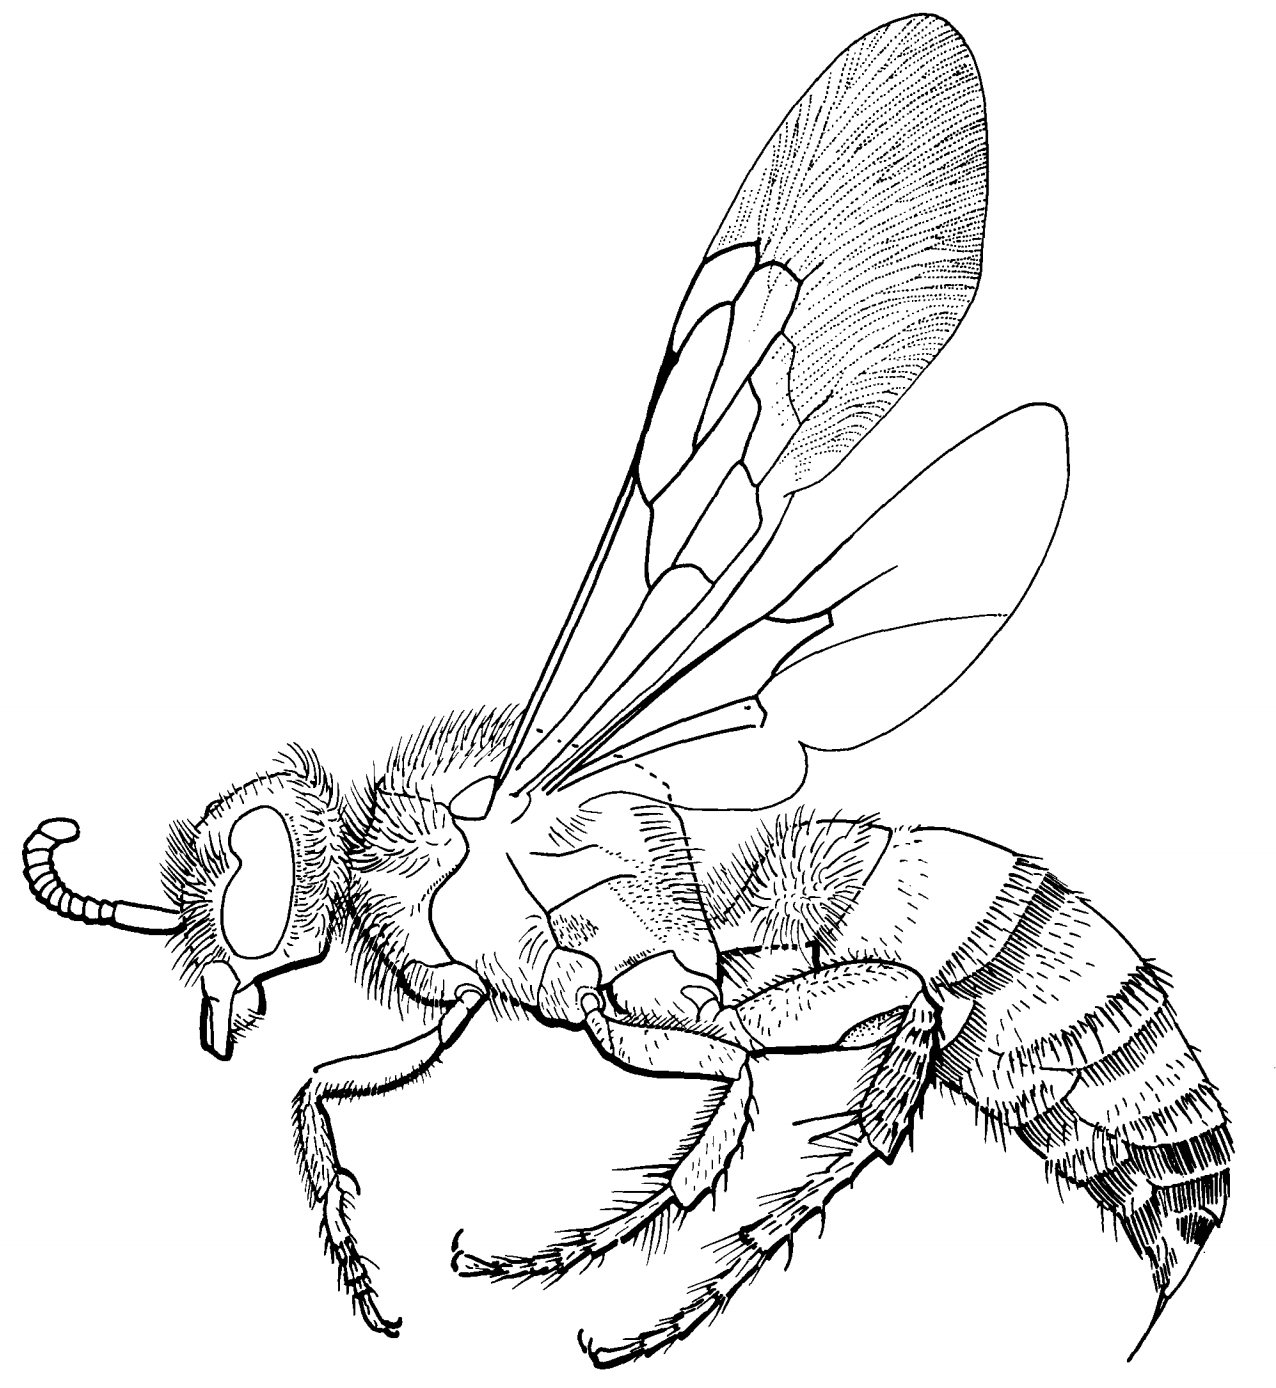
\includegraphics[width=\textwidth]{ScoliidHabitus}
        \caption{Habitus \citep[][Fig. 78]{goulet1993hymenoptera}}
        \label{fig:scoliid2}
    \end{subfigure}
    \caption{Scoliidae}\label{fig:scoliids}
\end{figure}

\subsubsection{Vespidae}
\noindent{}\textit{Diagnostic characters:} Eye with inner margin deeply emarginated; pronotum posterodorsal margin V-shaped, and with pronotum posterolateral apex acute and strongly produced above anterior margin of tegula; fore wing almost always longitudinally folded when at rest; hind wing without distinct claval lobe, and usually with distinct jugal lobe; posterior (inner) spur of metatibia weakly modified as a calcar; metasomal sternum 1 separated from sternum 2 by a deep constriction.\\

\noindent{}\textit{Natural history:} Many vespids are highly eusocial (You've probably encountered yellowjackets or bald-faced hornets here in Pennsylvania). Do you see any morphological evidence that these species are eusocial? Recall the question above for Formicidae.\\

\begin{figure}[ht!]
    \centering
    \begin{subfigure}[ht!]{0.25\textwidth}
        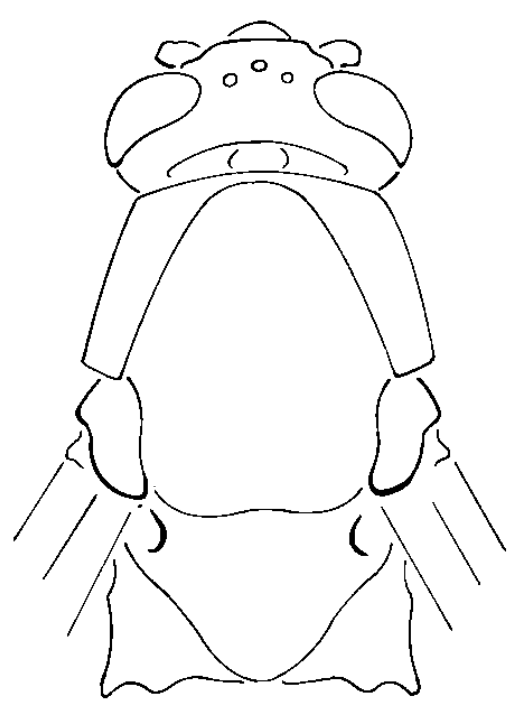
\includegraphics[width=\textwidth]{VespidMesosoma}
        \caption{Dorsal head and mesosoma \citep[][pg. 215]{goulet1993hymenoptera}}
        \label{fig:vespid1}
    \end{subfigure}
    \hfill
    \begin{subfigure}[ht!]{0.2\textwidth}
        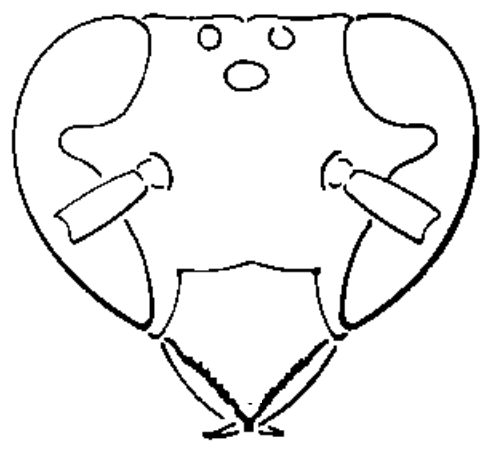
\includegraphics[width=\textwidth]{VespidHead}
        \caption{Anterior head \citep[][pg. 214]{goulet1993hymenoptera}}
        \label{fig:vespid2}
    \end{subfigure}
    \hfill
    \begin{subfigure}[ht!]{0.45\textwidth}
        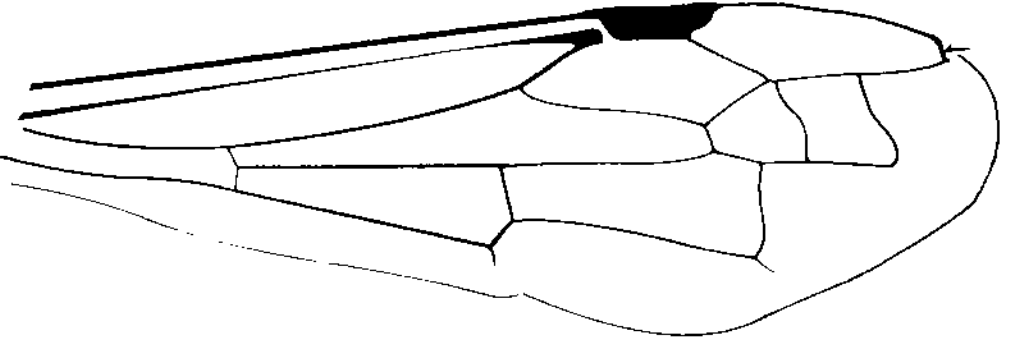
\includegraphics[width=\textwidth]{VespidWing}
        \caption{Fore wing \citep[][pg. 214]{goulet1993hymenoptera}}
        \label{fig:vespid3}
    \end{subfigure}
    \caption{Vespidae}\label{fig:vespids}
\end{figure}
\FloatBarrier

\noindent{}Now we're in Apoidea. This taxon comprises four families of spheciform wasps (we'll look at two), which are mostly predators of other insects, and seven to nine families of bees (Anthophila; we'll look at four bee families), which collect pollen. \\

\subsubsection{Sphecidae (thread-waisted, hunting wasps)}
\noindent{}\textit{Diagnostic characters:} Plumose, branched setae absent; hind leg basitarsus as wide as subsequent tarsomeres; metasoma petiolate (Figure \ref{fig:sphecid1}); first metasomal segment tube-like (sternum and tergum fused).\\

\noindent{}\textit{Natural history:} \\

\begin{figure}[ht!]
    \centering
    \begin{subfigure}[ht!]{0.45\textwidth}
        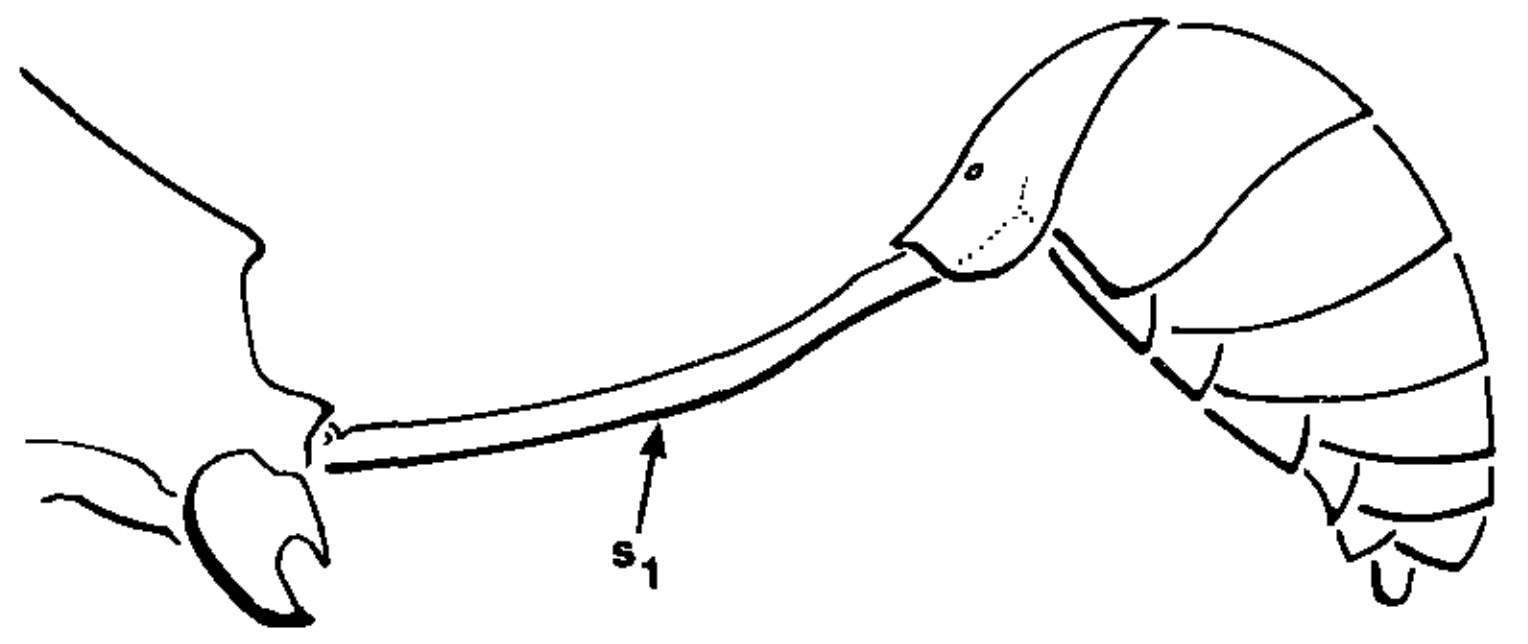
\includegraphics[width=\textwidth]{SphecidMetasoma}
        \caption{Mesasoma; s1 = sternite 1}
        \label{fig:sphecid1}
    \end{subfigure}
    \qquad
    \begin{subfigure}[ht!]{0.45\textwidth}
        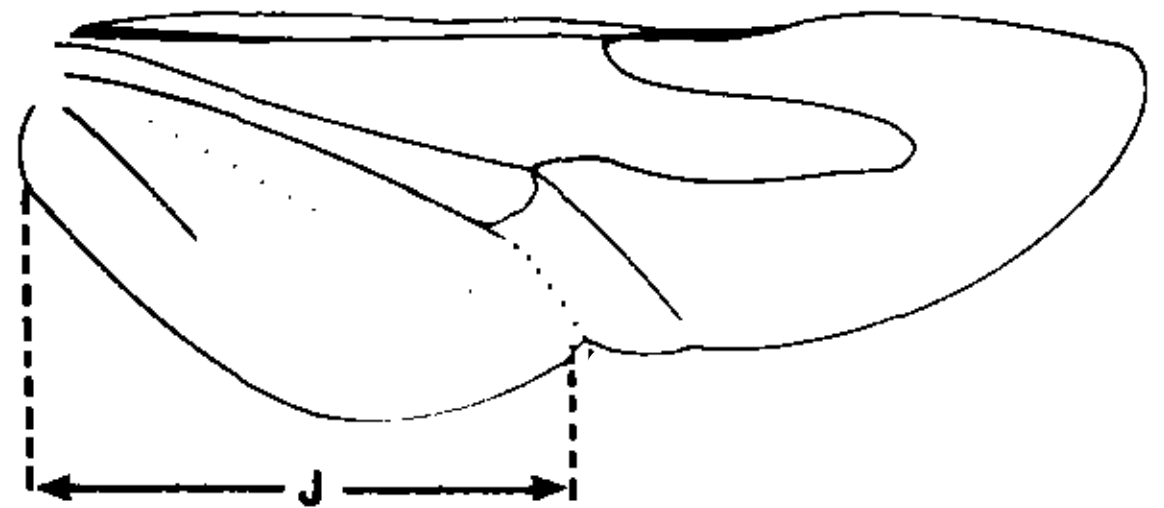
\includegraphics[width=\textwidth]{SphecidWing}
        \caption{Hind wing; J = jugal lobe}
        \label{fig:sphecid2}
    \end{subfigure}
    \caption{Sphecidae \citep[][pg. 281]{goulet1993hymenoptera}}\label{fig:sphecids}
\end{figure}

\subsubsection{Crabronidae (hunting wasps, aphid wasps, beewolves, cicada killers, \textit{etc}.)}
\noindent{}\textit{Diagnostic characters:} plumose, branched setae absent; hind leg basitarsus as wide as subsequent tarsomeres; tergum and sternum distinctly separated on metasomal segment 1; sometimes forming tube-like petiole; often determined through the process of elimination.\\

\noindent{}\textit{Natural history:} \\

\begin{figure}[ht!]
    \centering
    \begin{subfigure}[ht!]{0.4\textwidth}
        \includegraphics[width=\textwidth]{CrabronidHabitus1}
        \caption{Pemphredoninae habitus \citep[][Fig. 99]{goulet1993hymenoptera}}
        \label{fig:crabronid1}
    \end{subfigure}
    \qquad
    \begin{subfigure}[ht!]{0.4\textwidth}
        \includegraphics[width=\textwidth]{CrabronidHabitus2}
        \caption{Larrinae habitus \citep[][Fig. 102]{goulet1993hymenoptera}}
        \label{fig:crabronid2}
    \end{subfigure}
    \caption{Crabronidae}\label{fig:crabronids}
\end{figure}
\FloatBarrier

\noindent{}The remaining hymenopteran families are classified in \textbf{Anthophila} (bees). All have branched setae on the body and usually have (in females) some kind of pollen-carrying structure on the hind legs or abdomen.

\subsubsection{Halictidae (sweat bees)}
\noindent{}\textit{Diagnostic characters:} Hind leg basitarsus much wider than subsequent tarsomeres; face with one subantennal suture; proboscis short; jugal lobe of hind wing long; basal vein of fore wing strongly arched (Figure \ref{fig:halict1}); small to medium-sized, often metallic.\\

\noindent{}\textit{Natural history:} \\

\begin{figure}[ht!]
    \centering
    \begin{subfigure}[ht!]{0.26\textwidth}
        \includegraphics[width=\textwidth]{HalictidFace}
        \caption{Face \citep[][pg. 315]{goulet1993hymenoptera}}
        \label{fig:halict1}
    \end{subfigure}
    \qquad
    \begin{subfigure}[ht!]{0.4\textwidth}
        \includegraphics[width=\textwidth]{HalictidHabitus}
        \caption{Habitus \citep[][Fig. 118]{goulet1993hymenoptera}}
        \label{fig:halict2}
    \end{subfigure}
    \caption{Halictidae}\label{fig:halictidae}
\end{figure}

\subsubsection{Andrenidae (mining bees)}
\noindent{}\textit{Diagnostic characters:} Proboscis short; face with two subantennal sutures (Fig. \ref{fig:andrenid1}, double arrow) and often with facial foveae (Fig. \ref{fig:andrenid1}, single arrow); jugal lobe of hind wing long; basal vein of fore wing not strongly arched; small to medium-sized, often (not always!) with hairier thorax than halictids.\\

\noindent{}\textit{Natural history:} \\

\begin{figure}[ht!]
    \centering
    \begin{subfigure}[ht!]{0.24\textwidth}
        \includegraphics[width=\textwidth]{AndrenidFace}
        \caption{Head in anterior view \citep[][pg. 313]{goulet1993hymenoptera}}
        \label{fig:andrenid1}
    \end{subfigure}
    \qquad
    \begin{subfigure}[ht!]{0.37\textwidth}
        \includegraphics[width=\textwidth]{AndrenidHabitus}
        \caption{Habitus \citep[][Fig. 116]{goulet1993hymenoptera}}
        \label{fig:andrenid2}
    \end{subfigure}
    \caption{Andrenidae}\label{fig:andrenids}
\end{figure}

\subsubsection{Megachilidae (mason, leafcutter bees, \textit{etc}.)}
\noindent{}\textit{Diagnostic characters:} Proboscis rather long; jugal lobe of hind wing short; fore wing with two submarginal cells, usually equal in length; females with scopa (pollen carrier) on ventral surface of metasoma; variable in color and shape, but often stouter or ``chunkier'' than other bees.\\

\noindent{}\textit{Natural history:} \\

\begin{figure}[ht!]
    \centering
     \begin{subfigure}[ht!]{0.4\textwidth}
        \includegraphics[width=\textwidth]{MegachilidHabitus}
        \caption{Habitus \citep[][Fig. 116]{goulet1993hymenoptera}}
        \label{fig:megachilid1}
    \end{subfigure}
   \qquad
    \begin{subfigure}[ht!]{0.3\textwidth}
        \includegraphics[width=\textwidth]{ApidHabitus}
        \caption{Habitus \citep[][Fig. 123]{goulet1993hymenoptera}}
        \label{fig:apid1}
    \end{subfigure}
    \caption{}\label{fig:notused}
\end{figure}

\subsubsection{Apidae (cuckoo, nomad, carpenter, bumble, honey bees, \textit{etc}.)}
\noindent{}\textit{Diagnostic characters:} Tongue long, maxillary palps vestigial; jugal lobe of hind wing usually absent; fore wing with three submarginal cells; hind tibiae usually with a scopa used to carry pollen.\\

\noindent{}\textit{Natural history:} \\

\noindent{}As you have now seen, almost all bees are covered in plumose or branched setae and have special structures for carrying pollen. (Note: There are some species of cleptoparasitic bees that lack these structures.) Take a close look at the setae. Are they uniform in size and shape? How many specialized structures can you find on the body that you hypothesize might be involved in pollen collection? Based on the morphology, can you envision how pollen collection works from a behavioral perspective?

\FloatBarrier
% adding bibliography here
\bibliographystyle{apalike}
\bibliography{bib}

\end{document}

\subsubsection{Cimbicidae (cimbicid sawflies)}
\begin{itemize}
\item antennae with less than 7 flagellomeres, club=like
\item fore wing with 2 marginal cells 
\item two veins along the anteroproximal margin of fore wing connecting pterostigma with wing base
\item first abdominal tergum extending to metacoxa and fused with metapleuron
\end{itemize}

\subsubsection{Xiphydriidae (woodwasps)}
\begin{itemize}
\item antennae with \textgreater{}10 flagellomeres
\item mesonotum is divided by a straight transverse groove (Figure \ref{fig:xyiphid1})
\item two veins along the anteroproximal margin of fore wing connecting pterostigma with wing base
\end{itemize}

\subsubsection{Stephanidae}%replace with orussidae?
\begin{itemize}
\item head globular, with crown of ``teeth'' around median ocellus
\end{itemize}
\noindent{}These insects are parasitoids of wood-boring insects. What do you think they use the crown of teeth on the head for?

\subsubsection{Proctotrupidae}
\begin{itemize}
\item antenna not elbowed, with 12 antennomeres
\item fore wing with 2 cells enclosed by tubular veins (Figure \ref{fig:proctotrupid1}); can you see them?
\item medium size, usually black or brown
\end{itemize}

\subsubsection{Platygastridae}
\begin{itemize}
\item like Scelionidae except fore wing with no veins or with only one short proximal vein distant from anterior margin
\end{itemize}
